\documentclass[a4paper,oneside,11pt]{book}

\usepackage[italian]{babel}
\usepackage[utf8]{inputenc}
\usepackage{longtable}
\usepackage{verbatim}
\usepackage{amsthm}
\usepackage{amssymb}
\usepackage{amsfonts}
\usepackage{yhmath}
\usepackage[dvips]{graphicx}
\usepackage{makeidx}
\usepackage{wasysym}
\usepackage{pdfpages}


\theoremstyle{definition} \newtheorem{Def}{Definizione}
\theoremstyle{plain} \newtheorem{teo}{Teorema}
\theoremstyle{plain} \newtheorem{cor}[teo]{Corollario}
\theoremstyle{definition} \newtheorem{lem}[teo]{Lemma}
\theoremstyle{plain} \newtheorem{pro}[teo]{Proposizione}

\newcommand{\eqf}{\equiv}
\newcommand{\eqd}{\stackrel{\text{\textit{d}}}{=}}
\newcommand{\eqp}{\stackrel{\text{\textit{p}}}{=}}
\newcommand{\ug}[1]{(\ref{#1})} %ug sta per uguaglianza
\newcommand{\eqn}[1]{\stackrel{\text{\textit{#1}}}{=}}
\newcommand{\ud}{\,\mathrm{d}}

\title{Sul problema della misura e sulle decomposizioni paradossali negli spazi euclidei}
\author{Luca Franceschini}


\begin{document}

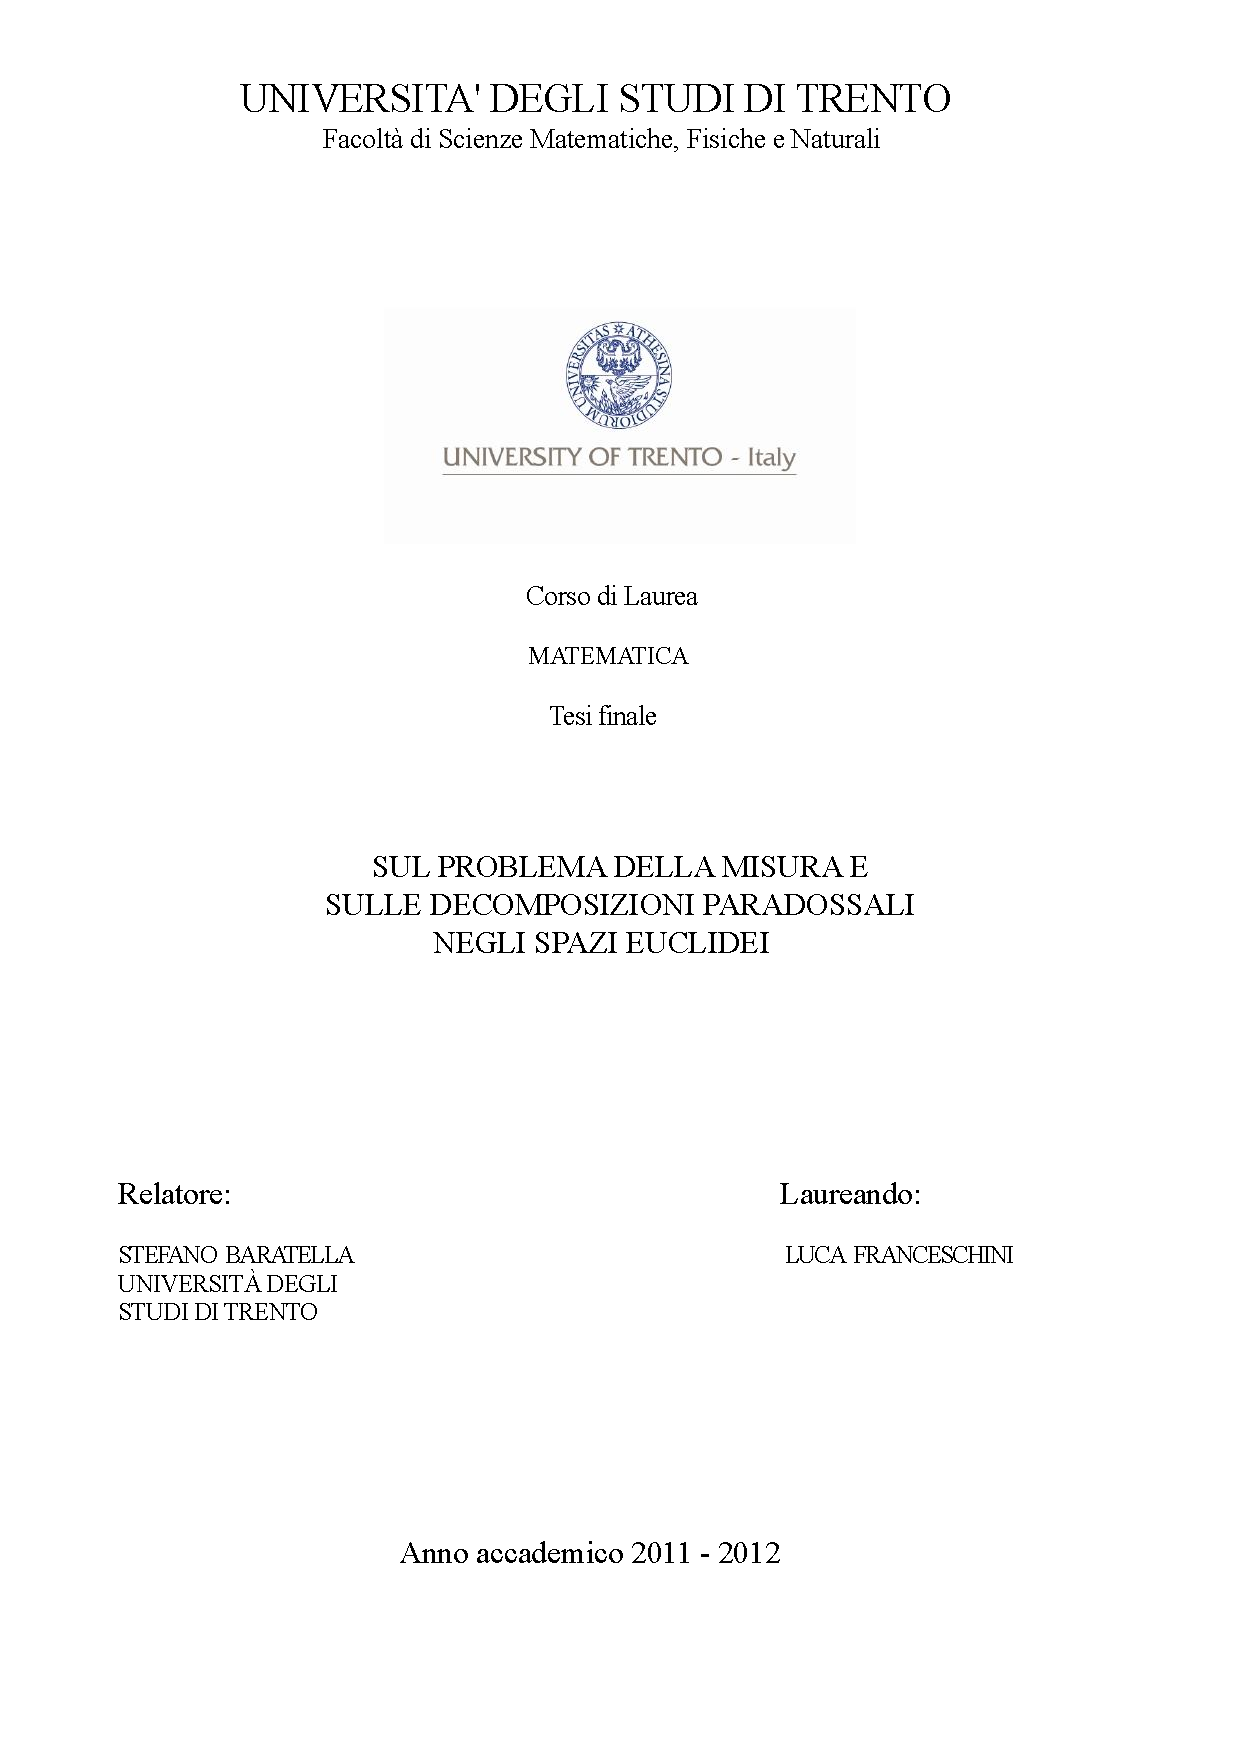
\includepdf[pages={1}]{Frontespizio.pdf}
\newpage\mbox{}\newpage
\tableofcontents


\chapter*{Introduzione}
\addcontentsline{toc}{chapter}{Introduzione}

	Una prima formulazione del problema della misura risale al 1902, quando Lebesgue scrisse nell'introduzione del libro \emph{Integrale, lunghezza, area} \cite{lebesgue}:
	\begin{quote}
		\emph{Ci proponiamo di associare ad ogni insieme limitato un numero positivo che chiameremo misura e soddisfacente le seguenti condizioni:
		\begin{enumerate}
			\item Esiste un insieme la cui misura non è nulla.
			\item Due insiemi uguali hanno la stessa misura.
			\item La misura dell'unione di in numero finito o di un infinità numerabile di insiemi, a due a due senza punti in comune, è la somma delle misure degli insiemi.
		\end{enumerate}}
	\end{quote}
	Questa descrizione corrisponde ad una misura numerabilmente additiva e invariante per traslazioni. La misura di Lebesgue è stata sviluppata assecondando questa idea, tuttavia Lebesgue non riuscì a dimostrare che la sua misura poteva essere usata per misurare tutti gli insiemi limitati in uno spazio euclideo.
	
	Nel 1905 Vitali dimostrò non solo che esistono insiemi che non sono Lebesgue-misurabili, ma anche che non esiste una misura numerabilmente additiva e invariante per traslazioni definita su tutti gli insiemi in uno spazio euclideo.
	
	Fu Hausdorff, nel 1914, a usare per la prima volta la locuzione ``problema della misura''\footnote{\emph{Das Problem der Inhaltbestimmung}, capitolo 10 in \cite{felix}.} nel libro \emph{Teoria degli insiemi}. Hausdorff si chiedeva se, rinunciando all'additività numerabile e chiedendo soltanto la finita additività, fosse possibile definire una misura invariante per isometrie per tutti gli insiemi limitati. In appendice dimostrò quello che ora è noto come Paradosso di Hausdorff, che implica la non esistenza di una misura finitamente additiva e invariante per traslazioni sulla sfera nello spazio euclideo tridimensionale.
	
	Nel 1923 Banach dedicò un articolo al problema della misura \cite{mesure} e dimostrò che esiste una misura finitamente additiva e invariante per traslazioni definita sugli insiemi limitati di retta e piano euclidei.
	
	Nel 1924 Banach e Tarski dimostrarono il loro celeberrimo paradosso per cui una palla può essere partizionata e ricomposta in due copie di sé stessa \cite{bantar}. Per la dimostrazione si servirono del Paradosso di Hausdorff. Da questo risultato segue che non può esistere una misura finitamente additiva e invariante per traslazioni per ogni spazio euclideo di dimensione $\geq 3$. Nello stesso articolo dimostrarono il risultato ancora più sorprendente per cui tutti gli insiemi con interno non vuoto nello spazio euclideo tridimensionale sono fra di loro equiscomponibili.
	
	Nel 1929 von Neumann generalizzò il problema della misura e lo affrontò per la prima volta dal punto di vista algebrico \cite{john}. Introducendo la nozione di \emph{gruppo ammissibile}, egli caratterizzò l'esistenza di decomposizioni paradossali in base al gruppo delle isometrie dello spazio euclideo considerato.

	\bigskip

	Questa tesi vuole essere una panoramica sul problema della misura e su alcune scoperte che sono seguite al suo studio.
	
	Nel capitolo 1 viene formulato il Problema della misura e dimostrato che non esiste una misura numerabilmente additiva definita su tutti gli insiemi limitati di uno spazio euclideo.
	
	Nel capitolo 2 vengono dimostrati il Paradosso di Hausdorff e il Paradosso di Banach-Tarski. Come corollario viene dimostrato che il problema della misura non ha soluzione negli spazi euclidei di dimensione $\geq 3$.
	
	Nel capitolo 3 viene introdotta la nozione di equiscomponibilità e dimostrata una generalizzazione del paradosso di Banach-Tarski.
	
	Nell'appendice vengono presentati, senza dimostrazione, alcuni risultati algebrici che risolvono il problema della misura su retta e piano euclidei. Più precisamente,  la soluzione positiva del problema della misura  è equivalente a una proprietà (detta \emph{ammissibilità}) del gruppo di isometrie dello spazio euclideo considerato.

\chapter{Formulazione del problema della misura}
\chaptermark{Problema della misura}
	
	In questo capitolo viene presentata la formulazione originale del problema della misura, proposta da Lebesgue \cite{lebesgue}. Viene poi esposta la dimostrazione di Hausdorff della sua irrisolvibilità \cite{felix}. Alla fine del capitolo viene dato l'enunciato definitivo del problema, che verrà poi approfondito nei capitolo successivi.
	
	\bigskip
	In questa tesi verrà denotato con $\mathbf{N}$ l'insieme dei numeri naturali $\geq 1$.
	\bigskip
	
	\begin{Def}
		Sia $n \in \mathbf{N}$. Lo \emph{spazio euclideo $n$-dimensionale} $\mathbf{E}^n$ è lo spazio vettoriale $\mathbf{R}^n$ equipaggiato col prodotto scalare standard:
		\begin{equation*}
			<\mathbf{x}, \mathbf{y}> = \sum_{i=1}^n x_i \cdot y_i \quad \forall\ \mathbf{x}, \mathbf{y} \in \mathbf{R}^n \text{.}
		\end{equation*}
		Su di esso si sottintende la struttura di spazio normato data dalla norma:
		\begin{equation*}
			||\mathbf{x}|| =  \sqrt{<\mathbf{x}, \mathbf{x}>} \quad \forall\ \mathbf{x} \in \mathbf{R}^n \text{,}
		\end{equation*}
		e la struttura di spazio metrico data dalla distanza:
		\begin{equation*}
			d(\mathbf{x}, \mathbf{y}) = ||\mathbf{x} - \mathbf{y}|| \quad \forall\ \mathbf{x}, \mathbf{y} \in \mathbf{R}^n \text{.}
		\end{equation*}
	\end{Def}
	
	\begin{Def}
		Sia $(X,d)$ uno spazio metrico. Due insiemi $A, B \subseteq X$ si dicono \emph{congruenti}, e si scrive $A \cong B$, se esiste una biiezione $f:X \to X$ tale che:
		\begin{itemize}
			\item $f(A) = f(B)$;
			\item $\forall x, y \in A \quad d(x,y) = d(f(x), f(y))$.
		\end{itemize}
	\end{Def}
	
	\begin{Def}\label{anello}
		Sia $X$ in insieme. Un \emph{anello} su $X$ è una famiglia di insiemi $\mathcal{A} \subseteq \mathcal{P}(X)$ tale che:
		\begin{itemize}
			\item $\varnothing \in \mathcal{A}$,
			\item $A,B\in \mathcal{A} \Rightarrow A \setminus B\in\mathcal{A}$,
			\item $A,B\in \mathcal{A} \Rightarrow A \cup B\in\mathcal{A}$,
			\item $A,B\in \mathcal{A} \Rightarrow A \cap B\in\mathcal{A}$.
		\end{itemize}
	\end{Def}
	
	Per ogni $n \in \mathbf{N}$ indicheremo con $\mathcal{L}_n$ la famiglia degli insiemi limitati in $\mathbf{E}^n$. Osserviamo che, per ogni $n \in \mathbf{N}$, $\mathcal{L}_n$ forma un anello.
	
	 \begin{Def}\label{defmis}
	 	Sia $\mathcal{A}$ un anello. Una \emph{misura finitamente additiva} su $\mathcal{A}$ è una funzione $m: \mathcal{A} \to [0, +\infty]$ non costantemente nulla tale che:%]]
	 	\begin{itemize}
	 		\item $m(\varnothing) = 0$,
	 		\item per ogni $n \in \mathbf{N}$, se $A_1, \dots, A_n \in \mathcal{A}$ sono a due a due disgiunti, allora $\sum\limits_{k=1}^n m(A_k) = m \left(\bigcup\limits_{k=1}^n A_k \right)$.
	 	\end{itemize}
	 	Una misura finitamente additiva $m$ è numerabilmente additiva se soddisfa la proprietà:
	 	\begin{itemize}
	 		\item se $\{A_k\}_{k \in \mathbf{N}} \subseteq \mathcal{A}$ è una famiglia di insiemi a due a due disgiunti e \\$\bigcup\limits_{k=1}^\infty A_k \in \mathcal{A}$, allora $\sum\limits_{k=1}^\infty m(A_k) = m\left(\bigcup\limits_{k=1}^\infty A_k\right)$.
	 	\end{itemize}
	 	In tal caso $m$ viene detta \emph{misura} tout court.
	\end{Def}
	
	Il problema della misura è stato formulato per la prima volta da Lebesgue nel 1902. Egli voleva generalizzare le usuali nozioni di lunghezza, area e volume a tutti gli insiemi limitati in uno spazio euclideo. Per questo aveva congetturato l'esistenza, per ogni spazio euclideo di ogni dimensione, di una funzione che chiameremo \emph{volume numerabilmente additivo}.
	
	\begin{Def}
		Sia $n \in \mathbf{N}$. Un \emph{volume numerabilmente additivo} su $\mathbf{E}^n$ è una funzione $f: \mathcal{L}_n \to [0, +\infty[$ tale che: %]]
	\begin{equation}\label{defprobmissba} %Definizione PROBlema della MISura SBAgliato
		\begin{aligned}
			&\text{(i) } f([0,1[^n) = 1 \text{;}\\%]]
			&\text{(ii) } \text{se } E_1 \cong E_2 \text{, allora } f(E_1) = f(E_2) \text{;}\\
			&\text{(iii) } f \text{ è numerabilmente additiva.}\\
		\end{aligned}
	\end{equation} 
	\end{Def}
	
	Le proprietà che caratterizzano un volume numerabilmente additivo sono quelle che appaiono ``naturali'' per una funzione che dovrebbe servire a ``misurare'' gli insiemi, infatti i volumi numerabilmente additivi sono delle misure nel senso della Definizione \ref{defmis}. 
	
	\begin{pro}\label{teomisvol} %Teorema MISura VOLume
		Sia $f$ un volume numerabilmente additivo su $\mathbf{E}^n$. Allora $f$ è una misura su $\mathcal{L}_n$.
	\end{pro}
	
	\begin{proof}
		È sufficiente provare che $f(\varnothing) = 0$. 
		
		Anzitutto, da (\ref{defprobmissba}.iii) segue facilmente che $f$ è monotona.
		
		Osserviamo che, per ogni $k \in \mathbf{N}$, la famiglia di insiemi
		\begin{equation*}
			\left\{ [ \frac{l}{k}, \frac{l+1}{k} [ \times [0,1[^{n-1}\ :\ l = 0, \dots, k-1 \right\}%]]
		\end{equation*}
		è una partizione di $[0,1[^n$. Inoltre gli insiemi di tale famiglia sono a due a due congruenti. Applicando tutte le proprietà elencate in \ug{defprobmissba} abbiamo che:
		\begin{equation*}
			1 = f([0,1[^n) = \sum_{l=0}^{k-1}  f\left( [\frac{l}{k}, \frac{l+1}{k}[ \times [0,1[^{n-1} \right) = k \cdot f\left([0,\frac{1}{k}[ \times [0,1[^{n-1}\right)\text{,}
		\end{equation*}
		da cui segue che, per ogni $k \in \mathbf{N}$:
		\begin{equation*}
			f\left([0,\frac{1}{k}[ \times [0,1[^{n-1}\right) = \frac{1}{k}\text{.}
		\end{equation*}
		
		Dalla monotonia di $f$ segue che, per ogni $k \in \mathbf{N}$, 
		\begin{equation*}
			f(\varnothing) \leq \frac{1}{k}\text{.}
		\end{equation*}
		Quindi $f(\varnothing) = 0$.
	\end{proof}
	
	Nel 1914 Hausdorff dimostrò che non esiste nessun volume numerabilmente additivo su $\mathbf{E}^n$, qualunque sia $n \in \mathbf{N}$. Di seguito riportiamo la dimostrazione di Hausdorff.		
	
	\begin{teo}\label{ncvg} %Non C'è Volume Generalizzato
		Per nessun $n \in \mathbf{N}$ esiste un volume numerabilmente additivo su $\mathbf{E}^n$.
	\end{teo}
	
	\begin{proof}
		È sufficiente provare che non esistono volumi n.a.\ su $\mathbf{E}^1$. Da ciò segue la non esistenza di un volume n.a.\ su spazi euclidei di dimensione maggiore. Infatti un volume n.a.\ $f$ su $\mathbf{E}^n$, per qualche $n >1$, induce un volume n.a.\ $\tilde{f}$ su $\mathbf{E}^1$ in questo modo:
		\begin{equation*}
			\tilde{f}(E) = f(E \times [0,1[^{n-1})\text{,}\quad E \in \mathcal{L}_1 \text{.} %]]
		\end{equation*}
		
		Supponiamo per assurdo che esista un volume n.a.\ $f$ su $\mathbf{E}^1$.
		
		Per ogni $x \in \mathbf{R}$ indicheremo con $\hat{x}$ il reale in $[0,1[$ tale che $\hat{x} = x + m$, per qualche $m \in \mathbf{Z}$. Se $A \subseteq \mathbf{R}$ indicheremo con $\hat{A}$ l'insieme degli $\hat{x}$, al variare di $x$ in $A$. %]]]]]]
		
		$\bullet$) Se $\alpha \in [0,1[$ e $A \subseteq [0,1[$, allora $f(A) = f(\widehat{A + \alpha})$.%]]]]]
		
		Sia $B = \widehat{A + \alpha}$. Poniamo:
		\begin{equation*}
			\begin{aligned}
				A_0 &= A \cap [0, 1-\alpha[ \text{ , }&\quad B_0 &= B \cap [\alpha, 1[ \text{ , }\\
				A_1 &= A \cap [1-\alpha, 1[ \text{ , }&\quad B_1 &= B \cap [0, \alpha[ \text{.}\\%]]]]]]]]
			\end{aligned}
		\end{equation*}
				
		Consideriamo le isometrie:
		\begin{equation*}
			\begin{aligned}
				\varphi_0:\ & \mathbf{R} \to \mathbf{R} \\
				&x \mapsto x + \alpha \\
			\end{aligned} \quad \text{ e } \quad \begin{aligned}
				\varphi_1:\ & \mathbf{R} \to \mathbf{R} \\
				&x \mapsto x + \alpha - 1 \\
			\end{aligned} \text{.}
		\end{equation*}
		Osserviamo che $\varphi_0(A_0) = B_0$ e $\varphi_1(A_1) = B_1$.	
		 
		Applicando (\ref{defprobmissba}.ii) e (\ref{defprobmissba}.iii) si ottiene:
		\begin{equation*}
			f(A) = f(A_0 \sqcup A_1) = f(A_0) + f(A_1) = f(B_0) + f(B_1) = f(B_0 \sqcup B_1) = f(B) \text{.}
		\end{equation*}
		
		$\bullet$) Fissiamo  un irrazionale $\alpha \in [0,1[$ e poniamo: %]]
		\begin{equation*}
			P_x = \{ \widehat{x + m\alpha} : m \in \mathbf{Z}\} \quad \text{per ogni } x \in [0, 1[ \text{.} %]]
		\end{equation*}
		Per definizione i $P_x$ sono a due due disgiunti oppure coincidenti.
		
		Con l'assioma di scelta otteniamo un insieme $A_0 \subseteq [0, 1[$ tale che $|A_0 \cap P_x| = 1$, per ogni $x \in [0,1[$. Per ogni $m \in \mathbf{Z}$ poniamo: %]]]]
		\begin{equation*}
			A_m = \{\widehat{x + m\alpha} : x \in A_0\} \text{.}
		\end{equation*}
		
		$\bullet$) Gli $A_m$ sono a due a due disgiunti oppure coincidenti.
		
		Vogliamo mostrare che se $A_m \cap A_n \neq \varnothing$, per qualche $m,n \in \mathbf{Z}$, allora $m = n$. Siano $x,y \in A_0$ e $m,n \in \mathbf{Z}$ tali che $\widehat{x+m\alpha} = \widehat{y + n\alpha}$. Abbiamo che:
		\begin{equation}\label{tiservoora}
			x = \hat{x} = \widehat{y + (n-m)\alpha} \text{ ;}
		\end{equation}
		segue che $P_x = P_y$ e quindi, per definizione di $A_0$, si ha che $x = y$. La \ug{tiservoora} diventa:
		\begin{equation*}
			x = \widehat{x + (n-m)\alpha} \text{,}
		\end{equation*}
		quindi, per qualche $k \in \mathbf{Z}$,
		\begin{equation*}
			x + k = x + (n - m) \alpha \text{.}
		\end{equation*}
		
		Se per assurdo $m \neq n$, allora $\alpha = \frac{k}{n-m}$, e quindi $\alpha$ sarebbe razionale. \lightning
		 
		$\bullet$) Osserviamo che:
		\begin{equation*}
			\bigcup_{m \in \mathbf{Z}} A_m = [0, 1[ \text{.} %]]
		\end{equation*}
		
		Per quanto mostrato nel primi due punti abbiamo che, per ogni $m \in \mathbf{Z}$:
		\begin{equation*}
			f(A_0) = f(A_m) \text{.}
		\end{equation*}
		Quindi, da (\ref{defprobmissba}), segue che:
		\begin{equation*}
				1 = f([0, 1[) = f\left(\bigcup_{m \in \mathbf{Z}} A_m\right) = \sum_{m \in \mathbf{Z}} f(A_m) = \sum_{m \in \mathbf{Z}} f(A_0) \text{.}%]]
		\end{equation*}
		Se $f(A_0)>0$, si avrebbe $\sum\limits_{m \in \mathbf{Z}} f(A_0) = +\infty$. Se invece $f(A_0) = 0$, si avrebbe $\sum\limits_{m \in \mathbf{Z}} f(A_0) = 0$. In entrambi i casi si ottiene una contraddizione.\lightning
	\end{proof}
	
	L'insieme di Vitali, definito per la prima volta nel 1905, è analogo all'insieme $A_0$ considerato nella dimostrazione del Teorema \ref{ncvg}. Usando l'assioma di scelta viene costruito un insieme che contiene una quantità numerabile di sottoinsiemi a due a due congruenti e disgiunti. Per dimostrare che l'insieme di Vitali non è Lebesgue-misurabile si deduce una contraddizione dall'invarianza per traslazioni e dall'additività numerabile della misura di Lebesgue, proprietà che possiedono anche i volumi numerabilmente additivi. 
	
	\bigskip
	
	Il Teorema \ref{ncvg} mostra che occorre rinunciare all'additività numerabile per rendere affrontabile il problema della misura. È stato Hausdorff a proporre la formulazione seguente che verrà approfondita nel resto della tesi.
	
	\begin{Def}\label{volume}
		Un \emph{volume} su $\mathbf{E}^n$ è una funzione $f: \mathcal{L}_n \to [0, +\infty[$ tale che:
		\begin{equation}\label{defpromis} %Definizione PROblema della MISura
			\begin{aligned}
				&\text{(i) } f([0,1[^n) = 1 \text{;}\\%]]
				&\text{(ii) } \text{se } E_1 \cong E_2 \text{, allora } f(E_1) = f(E_2) \text{;}\\
				&\text{(iii) } f \text{ è finitamente additiva.}\\
			\end{aligned}
		\end{equation}
	\end{Def}
	
	Con \emph{problema della misura} su $\mathbf{E}^n$ intendiamo l'esistenza di un volume su $\mathbf{E}^n$.
	
	\begin{pro}
		Per ogni $n \in \mathbf{N}$, un volume su $\mathbf{E}^n$ è una misura finitamente additiva su $\mathcal{L}_n$.
	\end{pro}
	\begin{proof}
		Analoga a quella della Proposizione \ref{teomisvol}.
	\end{proof}	
	
	\bigskip
	
	Il problema della misura può essere formulato in modo equivalente sostituendo la (\ref{defpromis}.i) con:
	\begin{equation}\label{ciao}
		f([0,1]^n) = 1 \text{.}
	\end{equation}
	Infatti si riesce a dimostrare facilmente che, per ogni $k \in \mathbf{N}$,
	\begin{equation*}
		f(]1-\frac{1}{k},1] \times [0,1]^{n-1}) \leq \frac{1}{k} \text{,}
	\end{equation*}
	da cui, per monotonia di $f$, segue che:
	\begin{equation*}
		f(\{1\} \times [0,1]^{n-1}) = 0 \text{.}
	\end{equation*}
	Analogamente si può dimostrare che, per ogni $k = 1, \dots, n-2$,
	\begin{equation*}
		f([0,1]^k \times \{1\} \times [0,1]^{n-k-1}) = 0 \text{,}
	\end{equation*}
	e che:
	\begin{equation*}
		f([0,1]^{n-1} \times \{1\}) = 0 \text{.}
	\end{equation*}
	Concludiamo che, sostituendo (\ref{defpromis}.i) con \ug{ciao},
	\begin{equation*}
		1 = f([0,1]^n) =
	\end{equation*}
	\begin{equation*}
		= f([0,1[^n) + f(\{1\} \times [0,1]^{n-1}) + \sum_{k=1}^{n-2} f([0,1]^k \times \{1\} \times [0,1]^{n-k-1}) + f([0,1]^{n-1} \times \{1\}) =
	\end{equation*}
	\begin{equation*}
		= f([0,1[^n) \text{.}
	\end{equation*}
	
	\bigskip
	
	Nel prossimo capitolo verrà mostrato che non esiste una soluzione al problema della misura per gli spazi euclidei di dimensione $\geq 3$. 
	
		 
\chapter{Decomposizione finita della sfera}
	
	In questo capitolo viene presentato e dimostrato il paradosso di Hausdorff \cite{felix}. Per alcune dimostrazioni è stato usato come riferimento \cite{strom}. Successivamente, mediante il paradosso di Hausdorff, viene dimostrato il paradosso di Banach-Tarski. La formulazione qui presentata è di Sierpinski \cite{sierp} ed è più forte dell'originale \cite{bantar}, perché specifica in quante parti va decomposta una palla in $\mathbf{E}^3$ per ottenerne due copie. Infine, come corollario, viene dimostrato che il problema della misura non ha soluzioni per spazi euclidei di dimensione maggiore di due.
	
\section{Paradosso di Hausdorff}
	
	Fissiamo $\theta \in [0, 2\pi[$ tale che $\cos \theta$ sia trascendente e consideriamo le matrici ortonormali: %]]
	\begin{equation}\label{phipsi}
		\varphi = \begin{pmatrix}
			-\cos\theta &0 &\sin\theta \\ \\
			0  &-1 &0 \\ \\
			\sin\theta &0 &\cos\theta \\
		\end{pmatrix} \quad \text{e} \quad \psi = \begin{pmatrix}
			 -\frac{1}{2} & -\frac{\sqrt{3}}{2} & 0 \\ \\
			 \frac{\sqrt{3}}{2} & -\frac{1}{2} & 0 \\ \\
			 0 & 0 & 1 \\
		\end{pmatrix} \text{.}
	\end{equation}
	
	La matrice $\varphi$ corrisponde ad una rotazione di $\pi$ attorno all'asse $\{(x,0,z) \in \mathbf{E}^3 : x \cos \frac{\theta}{2} = z \sin \frac{\theta}{2}\}$ e $\psi$ corrisponde ad una rotazione di $\frac{2}{3}\pi$ attorno all'asse $\{(0,0,z): z \in \mathbf{R}\}$.
	
	Sia $G$ il gruppo delle rotazioni in $\mathbf{E}^3$ generato da $\varphi$ e $\psi$. Per comodità poniamo $G^* = G \setminus \{\mathbf{1}\}$, dove $\mathbf{1}$ rappresenta la matrice identità $3 \times 3$. Valgono le seguenti:
	\begin{equation}\label{phipsi1}
		\varphi^2 = \psi^3 = \mathbf{1} \text{,}
	\end{equation}
	\begin{equation}\label{psi2}
		\psi^2 = \begin{pmatrix}
			-\frac{1}{2} &\frac{\sqrt{3}}{2} &0\\ \\
			-\frac{\sqrt{3}}{2} &-\frac{1}{2} &0\\ \\
			0 &0 &1\\
		\end{pmatrix} \text{.}
	\end{equation}
	
	Segue che ogni $\sigma \in G^*$ è scrivibile, per qualche $n \in \mathbf{N}$, come prodotto:
	\begin{equation}\label{esprsigma1} %ESPRessione SIGMA
		\sigma = \sigma_1 \dots \sigma_n \text{,}
	\end{equation}
	per qualche $\sigma_1, \dots, \sigma_n \in \{\varphi, \psi, \psi^2\}$ tali che, per ogni $i = 1, \dots, n-1$:
	\begin{equation}\label{esprsigma2}
		\sigma_i = \varphi \Rightarrow \sigma_{i+1} \in \{\psi, \psi^2\}\ \text{ e }\ \sigma_i \in \{\psi, \psi^2\} \Rightarrow \sigma_{i+1} = \varphi \text{.}
	\end{equation}
	Per ogni $\sigma \in G$ diremo che l'$n$-upla $(\sigma_1, \dots, \sigma_n)$ è un'\emph{espressione} di $\sigma$ se soddisfa \ug{esprsigma1} e \ug{esprsigma2}.
	
	In particolare ogni espressione di ciascun $\sigma \in G$ è di una delle seguenti forme:
	\begin{equation}\label{forph} %FORme Paradosso Hausdorff
	\begin{aligned}
		&(\alpha) &\sigma &= \prod_{i=1}^n  \psi^{m_i} \varphi &=\ &\psi^{m_1} \varphi \dots \psi^{m_n} \varphi \text{,}\\
		&(\beta) &\sigma &= \prod_{i=1}^n  \varphi \psi^{m_i} &=\ &\varphi \psi^{m_1} \dots \varphi \psi^{m_n} \text{,}\\
		&(\gamma) &\sigma &= \psi^{m_1} \prod_{i=2}^n  \varphi \psi^{m_i} &=\ &\psi^{m_1} \varphi \dots \varphi \psi^{m_n} \text{,}\\
		&(\delta) &\sigma &= \varphi  \prod_{i=1}^n \psi^{m_i}  \varphi &=\ &\varphi\psi^{m_1} \dots \psi^{m_n}\varphi \text{,}\\
	\end{aligned}
	\end{equation}
	dove $m_1, \dots, m_n \in \{1,2\}$.
	
	\begin{lem}\label{solo1nupla}
		Ogni $\sigma \in G^*$ ha un'unica espressione.
	\end{lem}
	
	\begin{proof}
		Procediamo per assurdo. Supponiamo che esistano, per qualche $n, m \in \mathbf{N}$, due espressioni $(\sigma_1, \dots, \sigma_n), (\rho_1, \dots, \rho_m)$ tali che:
		\begin{equation*}
			(\sigma_1, \dots, \sigma_n) \neq (\rho_1, \dots, \rho_m)\quad  \text{ e }\quad \sigma_1 \dots \sigma_n = \rho_1 \dots \rho_m \text{.}
		\end{equation*}
		
		Abbiamo che $\rho_m^{-1} \dots \rho_1^{-1} \sigma_1 \dots \sigma_n = \mathbf{1}$. L'$m$-upla $(\rho_m^{-1}, \dots, \rho_1^{-1})$ è a sua volta un'espressione, infatti:
		\begin{equation*}
			\rho_i^{-1} = \left\{\begin{aligned}
				&\varphi &\text{ se } \rho_i &= \varphi\\
				&\psi^2 &\text{ se } \rho_i &= \psi\\
				&\psi &\text{ se } \rho_i &= \psi^2\\
			\end{aligned}\right. \text{.}
		\end{equation*}
		A meno di semplificazioni abbiamo quindi ottenuto un'espressione di $\mathbf{1}$, oppure $m = n$ e $\sigma_i = \rho_i$ per ogni $i = 1, \dots, n$ (assurdo per ipotesi). Vogliamo mostrare che non esistono espressioni di $\mathbf{1}$.
		
		Procediamo per casi, distinguendo quelli elencati in \ug{forph}.
			
		$\bullet$) Sia $\sigma \in G$ come in (\ref{forph}.$\alpha$):
		\begin{equation*}
			\sigma = \psi^{m_1} \varphi \dots \psi^{m_n} \varphi \text{.}
		\end{equation*}
		La matrice $\sigma$ è il prodotto di $n$ fattori $\lambda_i = \psi^{m_i} \varphi$, scriviamo quindi $\sigma = \lambda_1 \dots \lambda_n$.
		Da \ug{phipsi} e \ug{psi2} segue che, a seconda di $m_i \in \{1, 2\}$, per ogni $i = 1, \dots, n$,
		\begin{equation*}
			\lambda_i = \begin{pmatrix}
				\frac{1}{2} \cos \theta &\pm \frac{\sqrt{3}}{2} &-\frac{1}{2} \sin \theta\\ \\
				\mp \frac{\sqrt{3}}{2} \cos \theta &\frac{1}{2} &\pm \frac{\sqrt{3}}{2} \sin \theta \\ \\
				\sin \theta &0 &\cos \theta\\
			\end{pmatrix} \text{.}
		\end{equation*}
		
		Mostriamo per induzione su $n \in \mathbf{N}$ che, per ogni $n$-upla $(\lambda_1, \dots, \lambda_n)$,
		\begin{equation*}
			\lambda_1 \dots \lambda_n \begin{pmatrix}
				0 \\ \\
				0 \\ \\
				1 \\
			\end{pmatrix} = \begin{pmatrix}
				\sin \theta \ x_{n-1}(\cos \theta)\\ 	\\
				\sqrt{3} \sin \theta \ y_{n-1}(\cos \theta) \\ \\
				z_n(\cos \theta)
			\end{pmatrix} \text{,}
		\end{equation*}
		per qualche $x_{n-1}(t), y_{n-1}(t) \in \mathbf{Q}[t]$ di grado $n-1$ e per qualche $z_n(t) \in \mathbf{Q}[t]$ di grado $n$.
		
		Se $n=1$, allora:
		\begin{equation*}
			\lambda_1 \begin{pmatrix}

				0 \\ \\
				0 \\ \\
				1 \\
			\end{pmatrix} = \begin{pmatrix}
				\sin \theta\ (-\frac{1}{2}) \\ \\
				\sqrt{3} \sin \theta\ (\pm\frac{1}{2}) \\ \\
				\cos \theta \\
			\end{pmatrix} \text{,}
		\end{equation*}
		che soddisfa la richiesta ponendo:
		\begin{equation*}
			x_0(t) = -\frac{1}{2} \text{,}\quad y_0(t) = \pm \frac{1}{2} \text{,}\quad z_1(t) = t \text{.}
		\end{equation*} 
		
		Se $n>1$, allora:
		\begin{equation*}
		\begin{aligned}
			\lambda_1 \dots \lambda_n \begin{pmatrix}
				0 \\ \\
				0 \\ \\
				1 \\
			\end{pmatrix} &= \lambda_1 (\lambda_2 \dots \lambda_n) \begin{pmatrix}

				0 \\ \\
				0 \\ \\

				1 \\
			\end{pmatrix}\\ \\
			&= \lambda_1 \begin{pmatrix}
				\sin \theta \ x_{n-2}(\cos \theta)\\ 	\\
				\sqrt{3} \sin \theta \ y_{n-2}(\cos \theta) \\ \\
				z_{n-1}(\cos \theta)
			\end{pmatrix}\\ \\
			&= \begin{pmatrix}
				\sin \theta\ \big[ \frac{1}{2} \cos \theta\ x_{n-2}(\cos \theta) \pm \frac{3}{4} y_{n-2}(\cos\theta)-\frac{1}{2} z_{n-1}(\cos\theta) \big]\\ \\
				\sqrt{3} \sin\theta\ \big[ \mp \frac{1}{2} \cos\theta\ x_{n-2}(\cos\theta) + \frac{1}{2} y_{n-2}(\cos\theta) \pm \frac{1}{2}z_{n-1}(\cos\theta)\big]\\ \\
				(1 - \cos^2 \theta)\ x_{n-2}\ (\cos\theta) + \cos\theta\ z_{n-1}(\cos\theta) \\
			\end{pmatrix} \text{,}\\
		\end{aligned}
		\end{equation*}
		che soddisfa la richiesta ponendo:
		\begin{equation*}
		\begin{aligned}
			x_{n-1}(t) &= \frac{1}{2}t \ x_{n-2}(t) \pm \frac{3}{4} y_{n-2}(t) - \frac{1}{2}z_{n-1}(t) \text{,}\\
			y_{n-1}(t) &= \mp \frac{1}{2}t\ x_{n-2}(t) + \frac{1}{2}y_{n-2}(t) \pm \frac{1}{2}z_{n-1}(t) \text{,}\\
			z_n(t) &= (1-t^2) x_{n-2}(t) + t \ z_{n-1}(t) \text{.}\\
		\end{aligned}
		\end{equation*}
		
		Se per assurdo, per qualche $n \in \mathbf{N}$, si può scrivere $\mathbf{1} = \lambda_1 \dots \lambda_n$, allora
		\begin{equation*}
			\lambda_1 \dots \lambda_n \begin{pmatrix}
				0\\ \\
				0\\ \\
				1\\
			\end{pmatrix} = \begin{pmatrix}
				0\\ \\
				0\\ \\
				1\\
			\end{pmatrix} \text{.}
		\end{equation*}
		Segue che:		
		\begin{equation*}
			p(\cos\theta) = 1 \quad \text{ per qualche $p(t) \in \mathbf{Q}[t]$ non costante,}
		\end{equation*}
		ma questo è impossibile, perché $\cos\theta$ è trascendente. \lightning
		
		$\bullet$) Se per assurdo $\mathbf{1}$ fosse esprimibile nella forma (\ref{forph}.$\beta$):
		\begin{equation*}
			\mathbf{1} = \varphi \psi^{m_1} \dots \varphi \psi^{m_n} \text{,}
		\end{equation*}
		si avrebbe:
		\begin{equation*}
			\mathbf{1} = \varphi^2 = \varphi \cdot \underbrace{\varphi \psi^{m_1} \dots \varphi\psi^{m_n}}_\mathbf{1} \cdot \varphi = \psi^{m_1} \varphi \dots \psi^{m_n} \varphi \text{,}
		\end{equation*}
		che è nella forma (\ref{forph}.$\alpha$). \lightning
		
		$\bullet$) Supponiamo per assurdo che $\mathbf{1}$ sia esprimibile nella forma (\ref{forph}.$\gamma$):
		\begin{equation*}
			\mathbf{1} = \psi^{m_1}\varphi \dots \varphi\psi^{m_n} \text{,}
		\end{equation*}
		con $n$ minimo tra i $k \in \mathbf{N}$ tali che $\mathbf{1} = \psi^{m_1}\varphi \dots \varphi\psi^{m_k}$.
		
		Ponendo:
		\begin{equation*}
			\bar{m_1} = \left\{\begin{aligned}
				1 \quad \text{ se } m_1 = 2\\
				2 \quad \text{ se } m_1 = 1\\
			\end{aligned} \right. \text{,}
		\end{equation*}
		si ha:
		\begin{equation*}
			\mathbf{1} = \psi^3 = \psi^{\bar{m_1}} \psi^{m_1} = \psi^{\bar{m_1}} \cdot \underbrace{\psi^{m_1}\varphi \dots \varphi\psi^{m_n}}_\mathbf{1} \cdot \psi^{m_1} = \varphi\psi^{m_2} \dots \varphi\psi^{m_n}\psi^{m_1} \text{,}
		\end{equation*}
		che è nella forma (\ref{forph}.$\beta$) se $m_1 + m_n \neq 3$. Nel caso in cui $m_1 + m_n = 3$, abbiamo che:
		\begin{equation*}
			\mathbf{1} = \varphi\psi^3\varphi = \varphi\psi^{m_n}\psi^{m_1}\varphi = \varphi\psi^{m_n} \cdot \underbrace{\psi^{m_1}\varphi \dots \varphi\psi^{m_n}}_\mathbf{1} \cdot \psi^{m_1}\varphi = \psi^{m_2}\varphi \dots \varphi\psi^{m_{n-1}} \text{,}
		\end{equation*}
		che è ancora nella forma (\ref{forph}.$\gamma$), contraddicendo la minimalità di $n$. \lightning
		
		$\bullet$) Se per assurdo $\mathbf{1}$ fosse esprimibile nella forma (\ref{forph}.$\delta$):
		\begin{equation*}
			\mathbf{1} = \varphi \psi^{m_1} \dots \psi^{m_n} \varphi \text{,}
		\end{equation*}
		si avrebbe:
		\begin{equation*}
			\mathbf{1} = \varphi^2 = \varphi \cdot \underbrace{\varphi \psi^{m_1} \dots \psi^{m_n} \varphi}_\mathbf{1} \cdot \varphi = \psi^{m_1} \varphi \dots \varphi \psi^{m_n} \text{,}
		\end{equation*}
		che è nella forma (\ref{forph}.$\gamma$). \lightning
		
	\end{proof}
		
	Legittimati dal Lemma precedente, diamo la seguente:
	\begin{Def}
		Sia $\sigma \in G^*$. Per qualche $n \in \mathbf{N}$ siano $\sigma_1, \dots, \sigma_n \in \{\varphi, \psi, \psi^2\}$ tali che:
		\begin{equation*}
			\sigma_1 \dots \sigma_n = \sigma
		\end{equation*}
		e, per ogni $i = 1, \dots, n-1$,
		\begin{equation*}
			\sigma_i = \varphi \Rightarrow \sigma_{i+1} \in \{\psi, \psi^2\}\ \text{ e }\ \sigma_i \in \{\psi, \psi^2\} \Rightarrow \sigma_{i+1} = \varphi \text{.}
		\end{equation*}
		Diremo che:
		\begin{itemize}
			\item $(\sigma_1, \dots, \sigma_n)$ è \emph{l}'espressione di $\sigma$,
			\item $\sigma$ ha \emph{lunghezza} $n$,
			\item $\sigma$ \emph{inizia} con $\sigma_1$.
		\end{itemize}
		
		Diremo che la matrice $\mathbf{1}$ ha lunghezza $0$.
	\end{Def}
	
	\begin{lem}
		Esiste una partizione $\{G_A, G_B, G_C\}$ di $G$ tale che, per ogni $\sigma \in G$:
		\begin{equation}\label{phpgp} %Paradosso Hausdorff Partizione G Proprietà
			\begin{aligned}
				&\text{(i) } &\sigma \in G_A & \Leftrightarrow \varphi\sigma \in G_B \cup G_C\\
				&\text{(ii) } &\sigma \in G_A & \Leftrightarrow \psi\sigma \in G_B\\
				&\text{(iii) } &\sigma \in G_A & \Leftrightarrow \psi^2\sigma \in G_C\\
			\end{aligned}
		\end{equation}
	\end{lem}
	
	\begin{proof}
		$\bullet$) Definiamo $G_A$, $G_B$, $G_C$ per induzione sulla lunghezza $n \in \mathbf{N}$ di $\sigma \in G$.
		
		Se $n = 0,1$ stabiliamo che:
		\begin{equation}\label{phpgd1} %Paradosso Hausdorff Partizione G Definizione
			\left\{\begin{aligned}
				&\mathbf{1} \in G_A \text{,}\\
				&\varphi, \psi \in G_B \text{,}\\
				&\psi^2 \in G_C \text{.}\\
			\end{aligned} \right. 
		\end{equation}
		
		Sia $n>1$. Se $\sigma \in G$ ha lunghezza $n-1$ e inizia con $\psi$ o $\psi^2$:
			\begin{equation}\label{phpgd2}
				\begin{aligned}
					&\text{(i) } \sigma \in G_B \cup G_C &\Rightarrow \varphi\sigma \in G_A \text{,}\\
					&\text{(ii) } \sigma \in G_A &\Rightarrow \varphi\sigma \in G_B \text{.}\\
				\end{aligned}
			\end{equation}
		Se $\sigma \in G$ ha lunghezza $n-1$ e inizia con $\varphi$:
			\begin{equation}\label{phpgd3}
				\begin{aligned}
					&\text{(i) } \sigma \in G_C \Rightarrow \psi\sigma \in G_A &\text{ e }\quad &\sigma \in G_B \Rightarrow \psi^2\sigma \in G_A \text{,}\\
					&\text{(ii) } \sigma \in G_A \Rightarrow \psi\sigma \in G_B &\text{ e }\quad &\sigma \in G_C \Rightarrow \psi^2\sigma \in G_B \text{,}\\
					&\text{(iii) } \sigma \in G_B \Rightarrow \psi\sigma \in G_C &\text{ e }\quad &\sigma \in G_A \Rightarrow \psi^2\sigma \in G_C \text{.}		
				\end{aligned}
			\end{equation}
			
		Per il Lemma precedente ogni $\sigma \in G$ appartiene ad esattamente un insieme della famiglia $\{G_A, G_B, G_C\}$. Segue che $\{G_A, G_B, G_C\}$ è una partizione di $G$ e che le implicazioni in \ug{phpgd2} e \ug{phpgd3} sono in realtà delle equivalenze.
		
		$\bullet$) Mostriamo per induzione sulla lunghezza $n \in \mathbf{N}$ di $\sigma \in G$ che \ug{phpgp} vale per ogni elemento di $G$.
		
		Se $n = 0$, allora $\sigma = \mathbf{1}$ e la \ug{phpgp} segue da \ug{phpgd1}.
		
		Se $n = 1$, allora $\sigma \in \{\varphi, \psi, \psi^2\}$. Osserviamo che $\{\varphi\psi, \varphi\psi^2, \psi^2\varphi\} \subseteq G_A$ e $\psi\varphi \in G_C$. Abbiamo che entrambi i membri di ogni equivalenza di \ug{phpgp} sono sempre falsi, quindi vale \ug{phpgp}.
		
		Sia $n>1$; procediamo per casi.
		
		$\diamond$) $\sigma$ inizia con $\varphi$
		
		Abbiamo che $\varphi\sigma$ inizia con $\psi$ o $\psi^2$. Da (\ref{phpgd2}.i) segue:
		\begin{equation*}
			\sigma = \varphi^2\sigma = \varphi(\varphi\sigma) \in G_A \Leftrightarrow \varphi\sigma \in G_B \cup G_C \text{,}
		\end{equation*}
		che equivale a (\ref{phpgp}.i).
		
		La (\ref{phpgp}.ii) e la (\ref{phpgp}.iii) seguono direttamente da, rispettivamente, (\ref{phpgd3}.ii) e (\ref{phpgd3}.iii).
		
		$\diamond$) $\sigma$ inizia con $\psi$
		
		La (\ref{phpgd2}.ii) è un caso particolare di (\ref{phpgp}.i).
		
		Abbiamo che $\psi\sigma = \psi^2\rho$, per qualche $\rho$ che inizia con $\varphi$. Da (\ref{phpgd3}.i) e (\ref{phpgd3}.ii) segue:
		\begin{equation*}
			\sigma = \psi\rho \in G_A \Leftrightarrow \rho \in G_C \Leftrightarrow \psi\sigma = \psi^2\rho \in G_B \text{,}
		\end{equation*}
		che equivale a (\ref{phpgp}.ii). Da (\ref{phpgd3}.i) segue:
		\begin{equation*}
			\sigma = \psi\rho \in G_A \Leftrightarrow \psi^2\sigma = \rho \in G_C \text{,}
		\end{equation*}
		che equivale a (\ref{phpgp}.iii).
	
		$\diamond$) $\sigma$ inizia con $\psi^2$
		
		La (\ref{phpgd2}.ii) è un caso particolare di (\ref{phpgp}.i).
		
		Abbiamo che $\psi\sigma = \psi^3\rho = \rho$, per qualche $\rho$ che inizia con $\varphi$. Da (\ref{phpgd3}.i) segue:
		\begin{equation*}
			\sigma = \psi^2\rho \in G_A \Leftrightarrow \psi\sigma = \rho \in G_B \text{,}
		\end{equation*}
		che equivale a (\ref{phpgp}.ii). Da (\ref{phpgd3}.i) e (\ref{phpgd3}.ii) segue:
		\begin{equation*}
			\sigma = \psi^2\rho \in G_A \Leftrightarrow \rho \in G_B \Leftrightarrow \psi^2\sigma = \psi\rho \in G_C \text{,}
		\end{equation*}
		che equivale a (\ref{phpgp}.iii).
	\end{proof}
	
	Il Teorema seguente è stato dimostrato da Hausdorff nel 1914 ed è alla base della dimostrazione del paradosso di Banach-Tarski esposta nel prossimo paragrafo.
	
	\begin{teo}[Paradosso di Hausdorff]\label{parhau} %PARadosso HAUsdorff
		Sia $S$ una sfera in $\mathbf{E}^3$ con centro nell'origine. Esiste una partizione $\{A, B, C, Q\}$ di $S$ tale che:
		\begin{equation*}
			\begin{aligned}
				&\text{i) } Q \text{ è numerabile} \text{,} &\quad &\text{ii) } \varphi(A) = B \cup C \text{,} \\
				&\text{iii) } \psi(A) = B  \text{,} &\quad &\text{iv) } \psi^2(A) = C \text{,} \\
				&\text{v) } \psi(Q) = \varphi(Q) = Q  \text{.} & \\
			\end{aligned}
		\end{equation*}
	\end{teo}
	
	\begin{proof}
		$\bullet$) (i) e (v)
		
		Poniamo:
		\begin{equation*}
			Q = \{\mathbf{x} \in S : \sigma(\mathbf{x}) = \mathbf{x} \text{ per qualche } \sigma \in G^*\} \text{.}
		\end{equation*}
		Vi sono tanti elementi in $G$ quante espressioni degli elementi di $G$, quindi $G$ è numerabile; ogni rotazione diversa dall'identità lascia fissi esattamente due punti, perciò anche l'insieme $Q$ è numerabile.
		
		Siano $\mathbf{x} \in Q$ e $\sigma \in G^*$ tali che $\sigma(\mathbf{x}) = \mathbf{x}$. Per ogni $\rho \in G^*$ abbiamo che $\rho\sigma\rho^{-1} (\rho(\mathbf{x})) = \rho(\mathbf{x})$, quindi anche $\varphi(\mathbf{x})$ e $\psi(\mathbf{x})$ appartengono a $Q$. Segue che $\varphi(Q) \subseteq Q$ e $\psi(Q) \subseteq Q$.
		
		Analogamente si può mostrare che, per ogni $\mathbf{x} \in Q$ e per ogni $\rho \in G^*$, $\rho^{-1}(\mathbf{x}) \in Q$. Segue che $Q \subseteq \varphi(Q)$ e $Q \subseteq \psi(Q)$.
		
		Concludiamo che $Q = \varphi(Q) = \psi(Q)$.
			
		$\bullet$) (ii), (iii) e (iv)
		
		Poniamo $P = S \setminus Q$ e, per ogni $\mathbf{x} \in P$:
		\begin{equation*}
			P_\mathbf{x} = \{\sigma(\mathbf{x}) : \sigma \in G\} \text{.}
		\end{equation*}
		
		Per definizione i $P_\mathbf{x}$ sono a due a due disgiunti oppure coincidenti. Mediante l'assioma di scelta otteniamo un insieme $M$ tale che $|P_\mathbf{x} \cap M| = 1$, per ogni $\mathbf{x} \in P$.
		
		Siano $\{G_A, G_B, G_C\}$ come nel Lemma precedente, poniamo:
		\begin{equation*}
			\begin{aligned}
				A &= \{\sigma(\mathbf{x}) : \sigma \in G_A\ \text{ e }\ \mathbf{x} \in M\} \text{,}\\
				B &= \{\sigma(\mathbf{x}) : \sigma \in G_B\ \text{ e }\ \mathbf{x} \in M\} \text{,}\\
				C &= \{\sigma(\mathbf{x}) : \sigma \in G_C\ \text{ e }\ \mathbf{x} \in M\} \text{.}\\
			\end{aligned}
		\end{equation*}
		Per il Lemma precedente e per definizione di $M$ si ha che $\{A, B, C\}$ è una partizione di $P$ tale che:
		\begin{equation*}
			\varphi(A) = B \cup C \text{ , } \quad \psi(A) = B\quad \text{ e } \quad \psi^2(A) = C \text{.}
		\end{equation*}
		
		Segue che $\{A, B, C, Q\}$ è una partizione con le proprietà richieste..
	\end{proof}
	
\section{Paradosso di Banach-Tarski}
	
	\begin{Def}
		Siano $X$ uno spazio metrico, $n \in \mathbf{N}$, $A,B \subseteq X$. Si dice che $A$ è \emph{equivalente a $B$ per $n$-decomposizione}, e si scrive $A \eqn{n} B$, se esistono due famiglie di insiemi a due a due disgiunti $\{A_1, \dots, A_n\}$ e $\{B_1, \dots, B_n\}$ tali che:
		\begin{itemize}
			\item per ogni $k = 1, \dots, n$, $A_k \cong B_k$,
			\item $\bigcup\limits_{k=1}^n A_k = A$ e $\bigcup\limits_{k=1}^n B_k = B$.
		\end{itemize}
	\end{Def}
	
	\begin{teo}\label{teobttb}\emph{\cite{ban24}}
		Siano $A$, $B$ insiemi e sia $A' \subseteq A$. Siano inoltre $\varphi: A \to B$ una mappa iniettiva e $\psi:A' \to B$ una biiezione.
		
		Esistono due insiemi disgiunti esaustivi $A_1, A_2 \subseteq A$ e due insiemi disgiunti esaustivi $B_1, B_2 \subseteq B$ tali che:
		\begin{equation*}
			\varphi(A_1) = B_1 \quad \text{e} \quad \psi(A_2) = B_2 \text{.}
		\end{equation*}
	\end{teo}
	
	\begin{proof}
		Se $A$ è vuoto, allora, per la biiettività di $\psi$, anche $B$ è vuoto. Se $B$ è vuoto, allora, per l'iniettività di $\varphi$, anche $A$ è vuoto. Quindi $A$ e $B$ sono entrambi vuoti o entrambi non vuoti.
		
		Se $A = B = \varnothing$, allora la tesi è ovvia. Assumiamo $A$ e $B$ non vuoti.
		
		Scriviamo $\varphi^{-1}$ per l'inversa della restrizione di $\varphi$ alla sua immagine.
		
		Per ogni $a \in A$ sia $C(a)$ il più piccolo $X \subseteq A$ tale che:
		\begin{equation}\label{bttb}
			\left\{\begin{aligned}
				&\text{(i) } a \in X \text{,}\\
				&\text{(ii) } \forall\ x \in X \quad \psi^{-1}\varphi(x) \in X \text{,}\\
				&\text{(iii) } \forall\ x \in X \quad \psi(x) \in \varphi(A) \Rightarrow \varphi^{-1}\psi(x) \in X \text{.}
			\end{aligned}\right.
		\end{equation}
		L'insieme $C(a)$ è ben definito, perché $A$ soddisfa \ug{bttb}.
		
		Siano $a_1, a_2 \in A$ tali che $C(a_1) \cap C(a_2) \neq \varnothing$ e sia $a \in C(a_1) \cap C(a_2)$. Gli insiemi $C(a_1)$, $C(a_2)$, $C(a)$ soddisfano (\ref{bttb}.ii), (\ref{bttb}.iii) e contengono $a$. Per la loro minimalità abbiamo che $C(a_1) = C(a) = C(a_2)$.
		
		Segue che gli insiemi della famiglia $\{C(a)\}_{a \in A}$ sono a due a due disgiunti o coincidenti.
		
		Sia $f$ una funzione con dominio contenuto nell'immagine. Per ogni $n \in \mathbf{N}$ indicheremo con $f^n$ la composizione $\underbrace{f \circ \dots \circ f}_{n \text{ volte}}$, intendendo con $f^0$ la mappa di inclusione.
		
		$ $\\
		$\bullet$) Per ogni $a \in A'$ proviamo che:\\
		se $\psi(a) \notin \varphi(A)$, allora:
		\begin{equation*}
			C(a) = \{a\} \cup \{(\psi^{-1}\varphi)^n(a) : n \in \mathbf{N}\} \text{.}
		\end{equation*}
		
		Sia $C'(a) = \{a\} \cup \{(\psi^{-1}\varphi)^n(a) : n \in \mathbf{N}\}$.
		
		L'inclusione $C'(a) \subseteq C(a)$ è immediata.
				
		Per mostrare che $C(a) \subseteq C'(a)$, dato che $a \in C'(a)$, è sufficiente provare (\ref{bttb}.ii) e (\ref{bttb}.iii).
		
		La (\ref{bttb}.ii) è immediata per definizione di $C'(a)$.
		
		Vogliamo provare che $C'(a)$ soddisfa (\ref{bttb}.iii). Sia $x \in C'(a)$.
		
		Se $x = a$, allora la premessa di (\ref{bttb}.iii) è falsa per ipotesi. Se $x = (\psi^{-1}\varphi)^n(a)$, per qualche $n>0$, allora $\psi(x) \in \varphi(A)$ e, inoltre,
		\begin{equation*}
			\varphi^{-1}\psi(x) = (\varphi^{-1}\psi)^{n-1}(a) \in C'(a) \text{.}
		\end{equation*}
				
		Quindi $C'(a)$ soddisfa (\ref{bttb}.iii).
		
		$\bullet$) Poniamo:
		\begin{equation*}
			\begin{aligned}
				A_2 &= \{a \in A : C(a) \subseteq A'\} \text{,}\\
				A_1 &= A \setminus A_2 \text{,}\\
				B_1 &= \varphi(A_1) \text{,}\\
				B_2 &= \psi(A_2) \text{.}
			\end{aligned}
		\end{equation*}
		
		Vogliamo provare che $B = B_1 \cup B_2$ e $B_1 \cap B_2 = \varnothing$. Ovviamente $B_1 \cup B_2 \subseteq B$.
		
		Sia $b \in B$. Distinguiamo due casi esaustivi ed opposti.
		
		$\diamond$) Proviamo che se $\psi^{-1}(b) \in A_1$, allora $b \in B_1$.
		
		Supponiamo $\psi^{-1}(b) \in A_1$. Se fosse che $b \notin \varphi(A)$, allora, per il punto predente,
		\begin{equation*}
			C\big(\psi^{-1}(b)\big) = \big\{\psi^{-1}(b)\big\} \cup \big\{(\psi^{-1}\varphi)^n\big(\psi^{-1}(b)\big) : n \in \mathbf{N}\big\} \subseteq \psi^{-1}(B) = A' \text{.}
		\end{equation*}
		Dunque $\psi^{-1}(b) \in A_2$: contraddizione. \lightning
		
		Concludiamo che $b \in \varphi(A)$. Sia $a \in A$ tale che $\varphi(a) = b$. Dato che $\psi^{-1}\varphi(a) = \psi^{-1}(b)$, abbiamo $C(a) = C\big(\psi^{-1}(b)\big)$, da cui $a \in A_1$. Quindi $b \in \varphi(A_1) = B_1$.
		
		$\diamond$) Se $\psi^{-1}(b) \in A_2$, allora $b \in \psi(A_2) = B_2$.
		
		Quindi $B_1$ e $B_2$ sono disgiunti e $B \subseteq B_1 \cup B_2$.
		
		Concludiamo che gli insiemi $A_1$, $A_2$, $B_1$ e $B_2$ soddisfano le proprietà richieste. 
	\end{proof}

	
	\begin{lem}\label{sierlemxyz}
		Siano $X,Y,Z$ sottoinsiemi di uno spazio metrico. Se $ X \supseteq Y \supseteq Z$ e $X \eqn{n} Z$, allora $X \eqn{n+1} Y$.
	\end{lem}
	
	\begin{proof}
		Per ipotesi esistono:
		\begin{itemize}
			\item una famiglia disgiunta esaustiva $\{X_1, \dots, X_n\}$ di $X$,
			\item una famiglia disgiunta esaustiva $\{Z_1, \dots, Z_n\}$ di $Z$,
			\item $k$ biiezioni $\varphi_1 : X \to X$, \dots, $\varphi_k : X \to X$,
		\end{itemize}
		tali che, per ogni $k =1, \dots, n$,
		\begin{equation}\label{sierlemxyz1} %SIERpinski Lemma X, Y, Z
			\varphi_k(X_k) = Z_k
		\end{equation}
		e, per ogni $x,y \in X_k$,
		\begin{equation}\label{sierlemxyz2}
			d(x,y) = d(\varphi_k(x), \varphi_k(y)) \text{.}
		\end{equation}
		
		Siano:
		\begin{equation*}
			\begin{aligned}
				\varphi: &X \to Z\\
				&x \mapsto \varphi_k(x)\ \text{ se $x \in X_k$, per $k = 1, \dots, n$}\\
			\end{aligned}
		\end{equation*}
		e $\psi = \text{id}_Y$.
		Osserviamo che $\varphi$ e $\psi$ sono biiezioni. Abbiamo che $\varphi(X) = Z \subseteq Y$ e $\psi(Y) = Y \subseteq X$. Per il Teorema \ref{teobttb} esistono una famiglia disgiunta esaustiva $\{X', X''\}$ di $X$ e una famiglia disgiunta esaustiva $\{Y', Y''\}$ di $Y$ tali che:
		\begin{equation*}
			\varphi(X') = Y' \quad \text{e} \quad X'' = \psi(X'') = Y'' \text{.}
		\end{equation*}
		
		La famiglia $\{X' \cap X_1, \dots, X' \cap X_n, X''\}$
		\begin{equation}\label{sierlemxyz3}
			\text{è una famiglia disgiunta esaustiva di $X$ con $n+1$ elementi.}
		\end{equation}
		
		Inoltre, $Y' = \varphi(X') \subseteq \varphi(X) = Z$, quindi $\{Y' \cap Y_1, \dots, Y' \cap Y_n, Y''\}$
		\begin{equation}\label{sierlemxyz4}
			 \text{è una  famiglia disgiunta esaustiva di $Y$ con $n+1$ elementi.}
		\end{equation}
		
		Dalla definizione di $\varphi$ e da \ug{sierlemxyz1} segue che, per ogni $k = 1, \dots, n$,
		\begin{equation*}
			\varphi(X' \cap X_k) = \varphi(X') \cap \varphi_k(X_k) = Y' \cap Z_k \text{,}
		\end{equation*}
		che, insieme a \ug{sierlemxyz2}, implica che:
		\begin{equation}\label{sierlemxyz5}
			\forall\ k = 1, \dots, n \quad X' \cap X_k \cong Y' \cap Z_k \text{.}
		\end{equation}
		
		Ovviamente $X'' \cong Y''$, quindi da \ug{sierlemxyz3}, \ug{sierlemxyz4}, \ug{sierlemxyz5} si conclude che:
		\begin{equation*}
			X \eqn{n+1} Y \text{.}
		\end{equation*}
	\end{proof}

	\begin{Def}
		Sia $n \in \mathbf{N}$ e siano $\mathbf{x},\mathbf{y} \in \mathbf{E}^n$. Il \emph{segmento} in $\mathbf{E}^n$ di \emph{estremi} $\mathbf{x}$ e $\mathbf{y}$ è l'insieme:
		\begin{equation*}
			]\mathbf{x}, \mathbf{y}[\ := \{t\mathbf{x} + (1-t)\mathbf{y} : 1 < t < 1\} \text{.}
		\end{equation*}
	\end{Def}
	
	Per $n=1$ la nozione di segmento è quella usuale di intervallo aperto.
	
	\begin{Def}
		Sia $n \in \mathbf{N}$. Siano $\mathbf{p} \in \mathbf{E}^n$ e $\rho \in ]0, +\infty[$. La \emph{palla} di \emph{centro} $\mathbf{p}$ e raggio $\rho$ è l'insieme:
		\begin{equation*}
			U = \{\mathbf{x} \in \mathbf{E}^n : ||\mathbf{x}-\mathbf{p}|| < \rho\} \text{.}
		\end{equation*}
		Con un'abuso di linguaggio chiameremo \emph{raggio} di $U$ qualsiasi segmento che abbia per estremi $\mathbf{p}$ ed un punto della frontiera di $U$.  
	\end{Def}
	
	Le frontiere delle palle sono sfere.
	
	\begin{lem}\label{sierlembt} %SIERpinski Lemma Banach Tarski
		Sia $U\subseteq \mathbf{E}^3$ una palla centrata nell'origine. Allora $U$ contiene due insiemi disgiunti $M$, $N$ tali che:
		\begin{equation*}
			M \eqn{2} U \quad \text{e} \quad N \eqn{5} U \text{.}
		\end{equation*}
	\end{lem}
	
	\begin{proof}
		Sia $S$ la frontiera di $U$ e siano $\varphi$, $\psi$ come nel Paragrafo 2.1. Possiamo applicare il Paradosso di Hausdorff (Teorema \ref{parhau}) ad $S$. Esiste quindi una partizione $\{A', B', C', Q'\}$ di $S$ tale che:
		\begin{equation*}
			Q' \text{ è numerabile} \text{,}
		\end{equation*}
		\begin{equation*}
			\varphi(A') = B' \cup C' \text{,} \quad \psi(A') = B' \text{,} \quad \psi^2(A') = C' \text{,}
		\end{equation*}
		\begin{equation*}
			\varphi(Q') = \psi(Q') = Q' \text{.}
		\end{equation*}
		
		Poniamo:
		\begin{equation*}
			\begin{aligned} %[
				A &= \bigcup_{\mathbf{x} \in A'} ]\mathbf{x}, \mathbf{0}[ \text{,} &\quad 
				B &= \bigcup_{\mathbf{x} \in B'} ]\mathbf{x}, \mathbf{0}[ \text{,} \\
				C &= \bigcup_{\mathbf{x} \in C'} ]\mathbf{x}, \mathbf{0}[ \text{,} &\quad
				Q &= \bigcup_{\mathbf{x} \in Q'} ]\mathbf{x}, \mathbf{0}[ \text{.} \\%]
			\end{aligned}
		\end{equation*}
		
		La famiglia $\{A, B, C, Q, \{\mathbf{0}\}\}$ è una partizione di $U$ tale che:
		\begin{equation*}
			\varphi(A) = B \cup C \text{,} \quad \psi(A) = B \text{,} \quad \psi^2(A) = C \text{,}
		\end{equation*}
		\begin{equation*}
			\varphi(Q) = \psi(Q) = Q \text{,} \quad \varphi(\{\mathbf{0}\}) = \psi(\{\mathbf{0}\}) = \{\mathbf{0}\} \text{.}
		\end{equation*}
		
		$\bullet$) Definiamo $M$ e una sua partizione $\{M_1, M_2\}$.
		
		Poniamo:
		\begin{equation*}
			\begin{aligned}
				M &= A \cup Q \cup \{\mathbf{0}\} \text{,}\\
				M_1 &= \varphi\psi(B) \text{,}\\
				M_2 &= \varphi\psi(M) \text{.}\\
			\end{aligned}
		\end{equation*}
		
		Gli insiemi $B$ ed $M$ sono disgiunti e $\varphi\psi$ è una biiezione, quindi,
		\begin{equation}\label{sierlembt1}
			M_1 \cap M_2 = \varnothing \text{.}
		\end{equation}
		
		Per definizione:
		\begin{equation*}
			\begin{aligned}
				\varphi\psi(A \cup B) &= \varphi(\psi(A) \cup \psi^2(A))\\
				&= \varphi(B \cup C)\\
				&= \varphi^2(A) = A \text{,} \\
				\varphi\psi(Q \cup \{\mathbf{0}\}) &= Q \cup \{\mathbf{0}\} \text{.} \\
			\end{aligned}
		\end{equation*}
		Quindi:
		\begin{equation}\label{sierlembt2}
			\begin{aligned}
				M_1 \cup M_2 &= \varphi\psi(B \cup M)\\
				&=\varphi\psi(A \cup B \cup Q \cup \{\mathbf{0}\})\\
				&= A \cup Q \cup \{\mathbf{0}\} = M \text{.}
			\end{aligned}
		\end{equation}
		
		Da \ug{sierlembt1} e \ug{sierlembt2} segue che
		\begin{equation}\label{sierlembt3}
			\{M_1, M_2\} \text{ è una partizione di } M \text{.}
		\end{equation}
		
		$\bullet$) Verifichiamo ora che $M \eqn{2} U$, usando le due partizioni $\{M_1, M_2\}$ e $\{A, B \cup C \cup Q \cup \{\mathbf{0}\}\}$.
		
		Per definizione si ha $M_1 = \varphi\psi^2(A)$, quindi:
		\begin{equation}\label{sierlembt4}
			M_1 \cong A \text{.}
		\end{equation}
		
		Sempre per definizione, si ha 
		\begin{equation*}
			\varphi\psi(A) = \varphi\psi\varphi(B \cup C) \quad  \text{e} \quad \varphi\psi(Q \cup \{\mathbf{0}\}) = \varphi\psi\varphi(Q \cup \{\mathbf{0}\}) \text{.}
		\end{equation*}
		Quindi:
		\begin{equation*}
			M_2 = \varphi\psi(A \cup Q \cup \{\mathbf{0}\}) = \varphi\psi\varphi(B \cup C \cup Q \cup \{\mathbf{0}\}) \text{,}
		\end{equation*}
		quindi:
		\begin{equation}\label{sierlembt5}
			M_2 \cong B \cup C \cup Q \cup \{\mathbf{0}\} \text{.}
		\end{equation}
		
		Da \ug{sierlembt3}, \ug{sierlembt4} e \ug{sierlembt5} segue che:
		\begin{equation*}
			M \eqn{2} U \text{.}
		\end{equation*}
		
		$\bullet$) Definiamo ora $N$ e una sua partizione $\{C_1, C_2, F_1, F_2, \{\mathbf{0}\}\}$.
		
		L'insieme $Q'$ è numerabile, quindi esiste un asse di rotazione che non passa per nessun punto di $Q'$. Sia $\mathcal{G}$ l'insieme delle rotazioni lungo tale asse e sia $\mathbf{x} \in Q'$. L'insieme $\{\beta \in \mathcal{G} : \beta(\mathbf{x}) \in Q'\}$ è al più equipotente a $Q'$. L'unione numerabile di insiemi numerabili è ancora numerabile, quindi l'insieme $\{\beta \in \mathcal{G} : \beta(Q') \cap Q' \neq \varnothing\}$ è al più numerabile. L'insieme $\mathcal{G}$ non è numerabile, quindi esiste $\alpha \in \mathcal{G}$ tale che $\alpha(Q') \cap Q' = \varnothing$. Abbiamo che $\alpha(Q) \cap Q = \varnothing$. Poniamo:
		\begin{equation*}
			E = \alpha(Q) \text{.} 
		\end{equation*}
		
		Allora:
		\begin{equation}\label{sierlembt6}
			E \subseteq A \cup B \cup C \quad \text{e} \quad E \cong Q \text{.} 
		\end{equation}
		
		Poniamo:
		\begin{equation*}
			\begin{aligned}
				F_1 &= \psi\varphi\psi^2(E) \cap \psi\varphi(C) \text{,} \\
				F_2 &= \psi\varphi\psi\varphi(E) \cap \psi\varphi(B) \text{,} \\
				F &= F_1 \cup F_2 \text{.} \\
			\end{aligned}
		\end{equation*}
		
		Per definizione si ha che $F_1 \subseteq \psi\varphi(C)$ e $F_2 \subseteq \psi\varphi(B)$. Dato che $B$ e $C$ sono disgiunti, si ha quindi che:
		\begin{equation}\label{sierlembt7}
			F_1 \cap F_2 = \varnothing \text{.} 
		\end{equation}
		
		Sempre per definizione:
		\begin{equation*}
			\psi\varphi(B \cup C) = \psi(A) = B \text{.} 
		\end{equation*}
		Quindi:
		\begin{equation*}
			F \subseteq B \text{.} 
		\end{equation*}
		Se per assurdo $F=B$, allora $B$ è un'unione numerabile di raggi. Da $A \cong B \cong C$ segue che anche $A$ e $C$ sono un'unione numerabile di raggi, quindi $U = A \cup B \cup C \cup Q$ è ancora un'unione numerabile di raggi. Si ottiene una contraddizione, perché $S$ non è numerabile. \lightning\\
		Possiamo quindi fissare $\mathbf{q} \in B \setminus F$.
		
		Poniamo:
		\begin{equation*}
			\begin{aligned}
				C_1 &= \psi^2\varphi(C) \text{,} \\
				C_2 &= \psi^2\varphi(B) \text{,} \\
				N &= C_1 \cup C_2 \cup F_1 \cup F_2 \cup \{\mathbf{q}\} \text{.} \\
			\end{aligned}
		\end{equation*}
		
		Dato che $B$ e $C$ sono disgiunti, si ha che:
		\begin{equation}\label{sierlembt8}
			C_1 \cap C_2 = \varnothing \text{.} 
		\end{equation}
		
		Inoltre, per definizione,
		\begin{equation*}
			F_1 \cup F_2 \cup \{\mathbf{q}\} \subseteq B \text{,} 
		\end{equation*}
		\begin{equation*}
			C_1 \cup C_2 = \psi^2\varphi(B \cup C) = \psi^2(A) = C \text{,} 
		\end{equation*}
		quindi:
		\begin{equation}\label{sierlembt9}
			(C_1 \cup C_2) \cap (F_1 \cup F_2 \cup \{\mathbf{q}\}) = \varnothing \text{.} 
		\end{equation}
		
		Da \ug{sierlembt7}, \ug{sierlembt8} e \ug{sierlembt9} segue che:
		\begin{equation}\label{sierlembt10}
			\{C_1, C_2, F_1, F_2, \{\mathbf{q}\}\} \text{ è una partizione di } N \text{.} 
		\end{equation}
		
		$\bullet$) Proviamo ora che $N \eqn{5} U$, usando le due partizioni $\{A, B \cup C, Q_1, Q_2, \{\mathbf{0}\}\}$ e $\{C_1, C_2, F_1, F_2, \{\mathbf{q}\}\}$.
		
		Per definizione:
		\begin{equation*}
			\begin{aligned}
				C_1 &= \psi^2\varphi\psi^2(A) \text{,} \\
				C_2 &= \psi^2\varphi\psi\varphi(B \cup C) \text{.} \\
			\end{aligned}
		\end{equation*}
		Quindi:
		\begin{equation}\label{sierlembt11}
			C_1 \cong A \quad  \text{e} \quad C_2 \cong B \cup C \text{.} 
		\end{equation}
		
		Poniamo:
		\begin{equation*}
			E_1 = E \cap A \quad \text{e} \quad E_2 = E \cap (B \cup C) \text{.} 
		\end{equation*}
		Per \ug{sierlembt6} esiste una partizione $\{Q_1, Q_2\}$ di $Q$ tale che:
		\begin{equation*}
			Q_1 \cong E_1 \quad \text{e} \quad Q_2 \cong E_2 \text{.} 
		\end{equation*}
		Per definizione, si ha che:
		\begin{equation*}
			\begin{aligned}
				\psi\varphi\psi^2(E_1) &= \psi\varphi\psi^2(E) \cap \psi\varphi\psi^2(A)\\
				&= \psi\varphi\psi^2(E) \cap \psi\varphi(C) = F_1 \text{,} \\
				\psi\varphi\psi\varphi(E_2) &= \psi\varphi\psi\varphi(E) \cap \psi\varphi\psi\varphi(B \cup C)\\
				&= \psi\varphi\psi\varphi(E) \cap \psi\varphi(B) = F_2 \text{.} \\
			\end{aligned}
		\end{equation*}
		Quindi:
		\begin{equation}\label{sierlembt12}
			F_1 \cong Q_1 \quad  \text{e} \quad F_2 \cong Q_2 \text{.} 
		\end{equation}
		
		La famiglia $\{A, B \cup C, Q_1, Q_2, \{\mathbf{0}\}\}$ è una partizione di $U$. Da \ug{sierlembt10}, \ug{sierlembt11} e \ug{sierlembt12} segue allora che:
		\begin{equation*}
			N \eqn{5} U \text{.}
		\end{equation*}
		
		$\bullet$) Verifichiamo infine che gli insiemi $M$ ed $N$ sono disgiunti. Infatti, per definizione,
		\begin{equation*}
			M = A \cup Q \cup \{\mathbf{0}\} \quad  \text{e} \quad N \subseteq B \cup C \text{.}
		\end{equation*}
	\end{proof}
	
	\begin{teo}[Paradosso di Banach-Tarski]\label{parbantar}
		Sia $U \subseteq \mathbf{E}^3$ una palla centrata nell'origine. Esiste una partizione $\{M, U \setminus M\}$ di $U$ tale che:
		\begin{equation*}
			M \eqn{2} U \quad  \text{e} \quad U \setminus M \eqn{6} U \text{.}
		\end{equation*}
	\end{teo}
	
	\begin{proof}
		Siano $M,N \subseteq U$ come nel Lemma \ref{sierlembt}. L'insieme $M$ soddisfa già la tesi. Inoltre abbiamo che $U \supseteq U \setminus M \supseteq N$ e $U \eqn{5} N$. Applicando il Lemma \ref{sierlemxyz}, si conclude che: $U \setminus M \eqn{6} U$.
	\end{proof}
	
	\begin{cor}
		Il problema della misura non ha soluzione per qualsiasi spazio euclideo di dimensione $\geq 3$.
	\end{cor}
	
	\begin{proof}
		Sia $n \geq 3$. Supponiamo per assurdo che la funzione $f: \mathcal{L}_n \to [0, +\infty[$ sia un volume su $\mathbf{E}^n$, secondo la definizione \ref{volume}. Distinguiamo due casi. %]]
		
		$\bullet$) $n = 3$
		
		Sia $U$ una palla contenente $[0,1[^3$. Da (\ref{defpromis}.i) segue che:
		\begin{equation*}
			f(U) \neq 0 \text{.}
		\end{equation*} 
		
		Sia $M$ come nel Teorema \ref{parbantar}.  Da (\ref{defpromis}.ii) segue che:
		\begin{equation*}
			f(U) = f(M) = f(U \setminus M) \text{.}
		\end{equation*}
		Applicando (\ref{defpromis}.iii) si ottiene:
		\begin{equation*}
			f(U) = f(M) + f(U \setminus M) = f(U) + f(U) \text{,}
		\end{equation*}
		che è assurdo, perché $f(U) \neq 0$. \lightning
		
		$\bullet$) $n > 3$
		 
		La funzione $\tilde{f}: \mathcal{L}_3 \to [0, +\infty[$ così definita:
		\begin{equation*}
			\tilde{f}(E) = f(E \times [0,1[^{n-3})\text{, } E \in \mathcal{L}_3 \text{,}
		\end{equation*}
		è un volume su $\mathbf{E}^3$, la cui esistenza contraddice il caso precedente. \lightning
	\end{proof}	
		
	
\chapter{Equiscomponibilità}

	In questo capitolo viene introdotta la nozione di equiscomponibilità. Dopo aver dimostrato che l'equiscomponibilità è una relazione di equivalenza, vengono presentati dei risultati che portano ad una generalizzazione del paradosso di Banach-Tarski. Non solo ogni palla in $\mathbf{E}^3$ è equiscomponibile a due copie di sé stessa, ma tutti gli insiemi limitati in $\mathbf{E}^3$ con interno non vuoto sono fra di loro equiscomponibili.
	
	Tutti i risultati in questo capitolo sono stati dimostrati da Banach e Tarski \cite{bantar} e alcuni di essi sono stati formulati in modo più forte da Sierpinski \cite{sierp}.

	\begin{Def}
		Sia $X$ uno spazio metrico. Due insiemi $A, B \subseteq X$ si dicono \emph{equiscomponibili}, e si scrive $A \eqf B$, se esiste $n \in \mathbf{N}$ tale che $A \eqn{n} B$.
	\end{Def}

	\begin{lem}\label{eqftra} %EQF TRAnsitiva
		Sia $X$ uno spazio metrico e siano $A, B, C \subseteq X$. Se $A \eqf B$ e $B \eqf C$, allora $A \eqf C$.
	\end{lem}
	
	\begin{proof}
		Sia $n \in \mathbf{N}$ tale che esistono due famiglie di insiemi a due a due disgiunti $\{A_1, \dots, A_n\}$,  $\{B_1, \dots, B_n\}$ ed una biiezione $\varphi: A \to B$ tali che:
		\begin{itemize}
			\item $\bigcup\limits_{k=1}^n A_k = A$ e $\bigcup\limits_{k=1}^n B_k = B$,
		\end{itemize}
		e, per ogni $k = 1, \dots, n$,
		\begin{itemize}
			\item $\varphi(A_k) = B_k$,
			\item per ogni $x,y \in A_k$, $d(x, y) = d(\varphi(x), \varphi(y))$.
		\end{itemize}
	
		Analogamente, sia $m \in \mathbf{N}$ tale che esistono due famiglie di insiemi a due a due disgiunti $\{B'_1, \dots, B'_m\}$, $\{C_1, \dots, C_m\}$ ed una biiezione $\psi: B \to C$ tali che:
		\begin{itemize}
			\item $\bigcup\limits_{l=1}^m B'_l = B$ e $\bigcup\limits_{l=1}^m C_l = C$,
		\end{itemize}
		e, per ogni $l = 1, \dots, m$,
		\begin{itemize}
			\item $\psi(B'_l) = C_l$,
			\item per ogni $x,y \in B'_l$, $d(x, y) = d(\psi(x), \psi(y))$.
		\end{itemize}
	
		Per ogni $k = 1, \dots, n$ e per ogni $l = 1, \dots, m$ poniamo:
		\begin{equation*}
			\tilde{A}_{k,l} = \varphi^{-1}(\psi^{-1}(C_l) \cap B_k) \quad \text{e} \quad \tilde{C}_{k,l} = (\psi \circ \varphi)(\tilde{A}_{k,l}) \text{.}
		\end{equation*}
	
	
		Consideriamo le seguenti famiglie di insiemi a due a due disgiunti:
		\begin{equation*}
			\begin{aligned}
				\mathcal{A} &= \{ \tilde{A}_{k,l} : k = 1, \dots, n\ \text{ e }\ l = 1, \dots, m \} \quad \text{e}\\
				\mathcal{C} &= \{ \tilde{C}_{k,l} : k = 1, \dots, n\ \text{ e }\ l = 1, \dots, m \} \text{.}\\
			\end{aligned}
		\end{equation*}
	
		Abbiamo che $\bigcup\mathcal{A} = A$ e $\bigcup\mathcal{C} = C$. Concludiamo mostrando che, per ogni $k = 1, \dots, n$ e per ogni $l = 1, \dots, m$, $\tilde{A}_{k,l} \cong \tilde{C}_{k,l}$.
	
		Le funzioni $\varphi$ e $\psi$ sono entrambe biiettive, quindi anche la loro composizione $\psi \circ \varphi$ è ancora biiettiva.
	
		Per definizione $\tilde{A}_{k,l} \subseteq \varphi^{-1}(B_k) = A_k$, quindi:
		\begin{equation*}
			\forall\ x,y \in \tilde{A}_{k,l} \quad d(x, y) = d(\varphi(x), \varphi(y)) \text{.}
		\end{equation*}
		Sempre per definizione $\varphi(\tilde{A}_{k,l}) \subseteq \psi^{-1}(C_l) = B'_l$, quindi:
		\begin{equation*}
			\forall\ x,y \in \tilde{A}_{k,l} \quad d(x, y) = d\Big((\psi \circ \varphi)(x), (\psi \circ \varphi)(y)\Big) \text{.}
		\end{equation*}
	
		Segue che la restrizione di $\psi \circ \varphi$ a $\tilde{A}_{k,l}$ è un'isomorfismo di spazi metrici di $\tilde{A}_{k,l}$ su $\tilde{C}_{k,l}$. Quindi $\tilde{A}_{k,l} \cong \tilde{C}_{k,l}$, per ogni $k = 1, \dots, n$, $l = 1, \dots, m$.
	\end{proof}

	\begin{cor}
		L'equiscomponibilità è una relazione d'equivalenza.
	\end{cor}
	
	\begin{proof}
		Riflessività e simmetria sono immediate. La transitività è garantita dal Lemma \ref{eqftra}.
	\end{proof}
	
	\begin{pro}\label{akbkaeqfb} %A_K B_K implica A EQF B
		Sia $X$ uno spazio metrico e siano $A,B \subseteq X$. Sia $n \in \mathbf{N}$ e siano $\{A_1, \dots, A_n\}$ e $\{B_1, \dots, B_n\}$ due famiglie di insiemi a due a due disgiunti tali che $\bigcup\limits_{k=1}^n A_k = A$ e $\bigcup\limits_{k=1}^n B_k = B$. Se, per ogni $k = 1, \dots, n$,
		\begin{equation*}
			A_k \eqf B_k \text{,}
		\end{equation*}
		allora $A \eqf B$.
	\end{pro}
	
	\begin{proof}
		Per ogni $k = 1, \dots, n$ sia $m_k \in \mathbf{N}$ per cui esistono due famiglie di insiemi a due a due disgiunti $\{A'_{k,1}, \dots, A'_{k,m_k}\}$, $\{B'_{k,1}, \dots, B'_{k,m_k}\}$ tali che: $\bigcup\limits_{l=1}^{m_k} A'_{k,l} = A$, $\bigcup\limits_{l=1}^{m_k} B'_{k,l} = B$, e
		\begin{equation}\label{akbkaeqfb1}
			\forall\ l = 1, \dots, m_k \quad A'_{k,l} \cong B'_{k,l} \text{.}
		\end{equation}
		
		Poniamo:
		\begin{equation*}
			\mathcal{A} = \{A'_{k,l} : k = 1, \dots, n \quad \text{e} \quad l = 1, \dots, m_k\} \quad\text{e}
		\end{equation*}
		\begin{equation*}
			\mathcal{B} = \{B'_{k,l} : k = 1, \dots, n \quad \text{e} \quad l = 1, \dots, m_k\} \text{.}
		\end{equation*}
		
		Gli insiemi nelle famiglie $\mathcal{A}$ e $\mathcal{B}$ sono a due a due disgiunti e:
		\begin{equation*}
			\begin{aligned}
				\bigcup \mathcal{A} &= \bigcup_{k=1}^n \bigcup_{l=1}^{m_k} A'_{k,l} = \bigcup_{k=1}^n A_k = A \text{,}\\
				\bigcup \mathcal{B} &= \bigcup_{k=1}^n \bigcup_{l=1}^{m_k} B'_{k,l} = \bigcup_{k=1}^n B_k = B \text{.}\\
			\end{aligned}
		\end{equation*}
		Da \ug{akbkaeqfb1} segue immediatamente che $A \eqf B$.
	\end{proof}
	
	\begin{pro}\label{aeqfbcadb}%A EQF B, C in A e D in B
		Sia $X$ uno spazio metrico e siano $A, B \subseteq X$. Se $A \eqf B$, allora per ogni $C \subseteq A$ esiste $D \subseteq B$ tale che:
		\begin{itemize}
			\item $C \eqf D$,
			\item se $C \neq A$, allora $D \neq B$.
		\end{itemize}
	\end{pro}
	
	\begin{proof}
		Sia $n \in \mathbf{N}$ per cui esistono due famiglie di insiemi a due a due disgiunti $\{A_1, \dots, A_n\}, \{B_1, \dots, B_n\}$ tali che $\bigcup\limits_{k=1}^n A_k = A$, $\bigcup\limits_{k=1}^n B_k = B$ e
		\begin{equation}\label{aeqfbcadb1}
			\forall\ k = 1, \dots, n \quad A_k \cong B_k \text{.}
		\end{equation}
		
		Per ogni $k= 1, \dots, n$ sia $\varphi_k : A_k \to B_k$ un isomorfismo di spazi metrici. Poniamo:
		\begin{equation*}
			\begin{aligned}
				&\varphi: &A &\to B\\
				& &p &\mapsto \varphi_k (p) \quad \text{se  $p \in A_k$, per $k = 1, \dots, n$.}
			\end{aligned}
		\end{equation*}
		
		La mappa $\varphi$ è ben definita ed è una biiezione.
		
		Fissiamo $C \subseteq A$ e poniamo, per ogni $k = 1, \dots, n$,
		\begin{equation*}
			C_k = C \cap A_k \text{.}
		\end{equation*}

		Per ogni $k = 1, \dots, n$ le restrizioni $\varphi_k: C_k \to \varphi(C_k)$ sono degli isomorfismi di spazi metrici, quindi:
		\begin{equation}\label{aeqfbcadb2}
			C_k \cong \varphi(C_k) \text{.}
		\end{equation}
		
		Poniamo $D = \varphi(C)$. Si ha che $\{C_1, \dots, C_n\}$ e $\{\varphi(C_1), \dots, \varphi(C_n)\}$ sono famiglie esaustive di insiemi a due a due disgiunti rispettivamente di $C$ e $D$. Quindi, da \ug{aeqfbcadb2} si conclude che: $C \eqf D$.
		
		Il secondo punto della tesi segue dalla biiettività di $\varphi$.
	\end{proof}
	
	\begin{lem}\label{eqfabc} %EQF A, B, C
		Sia $X$ uno spazio metrico e siano $A, B, C \subseteq X$. Se $A \supseteq B \supseteq C$ e $A \eqf C$, allora $A \eqf B$.
	\end{lem}
	
	\begin{proof}
		Sia $n \in \mathbf{N}$ tale che $A \eqn{n} C$. Applicando il Lemma \ref{sierlemxyz} del capitolo 3 si ottiene: $A \eqn{n+1} B$, quindi $A \eqf B$.
	\end{proof}
	
	\begin{pro}\label{aubkaub} %A U B_K A U B
		Sia $X$ uno spazio metrico. Sia $A \subseteq X$ e siano $B_1, \dots, B_n \subseteq X$ tali che
		\begin{equation*}
			\forall\ k = 1, \dots, n \quad A \eqf A \cup B_k \text{.}
		\end{equation*}
		Allora
		\begin{equation*}
			A \eqf A \cup \bigcup_{k=1}^n B_k \text{.}
		\end{equation*}
	\end{pro}
	
	\begin{proof}
		Procediamo per induzione su $n$.
		
		Se $n=1$, la tesi è ovvia.
		
		Sia $n>1$; distinguiamo due casi.
		
		$\bullet$) Gli insiemi $A, B_1, \dots, B_n$ sono a due a due disgiunti.

		Abbiamo che: $A \eqf A \cup B_1 \cup \dots \cup B_{n-1}$ e $A \eqf A \cup B_n$. Applicando la Proposizione \ref{akbkaeqfb} alle famiglie $\{A, B_n\}$ e $\{A \cup B_1 \cup \dots \cup B_{n-1}, B_n\}$ otteniamo:
		\begin{equation*}
		 	A \cup B_n \eqf \big(A \cup B_1 \cup \dots \cup B_{n-1} \big) \cup B_n = A \cup B_1 \cup \dots \cup B_n \text{,}
		\end{equation*}
		da cui:
		\begin{equation*}
			A \eqf A \cup B_n \eqf A \cup B_1 \cup \dots \cup B_n \text{.}
		\end{equation*}
		 
		$\bullet$) Caso generale.
		 
		Poniamo:
		\begin{equation*}
			\left\{\begin{aligned}
				B'_1 &= B_1 \setminus A \text{,}\\
				B'_k &= B_k \setminus \big(A \cup B_1 \cup \dots \cup B_{k-1}\big)\quad  \text{se } 1 < k \leq n \text{.}\\
			\end{aligned}\right.
		\end{equation*}
		
		Osserviamo che, per ogni $k = 1, \dots, n$, $A \subseteq A \cup B'_k \subseteq A \cup B_k$. Applichiamo il Lemma \ref{eqfabc} e otteniamo $A \eqf A \cup B'_k$.
		
		Per definizione gli insiemi $A, B'_1, \dots, B'_n$ sono a due a due disgiunti, quindi, applicando il caso precedente, abbiamo la tesi:
		\begin{equation*}
			A \eqf A \cup B'_1 \cup \dots \cup B'_n = A \cup B_1 \cup \dots \cup B_n \text{.}
		\end{equation*}
		 
	\end{proof}
	
	\begin{lem}\label{u1u2eqfu1uu2} %U1 U2 EQF U1 U U2
		Se $U_1, U_2 \subseteq \mathbf{E}^3$ sono due palle congruenti (non necessariamente disgiunte), allora $U_1 \eqf U_1 \cup U_2$.
	\end{lem}
	
	\begin{proof}
		Per il Lemma \ref{sierlembt} esistono due insiemi disgiunti $A_1, A_2 \subseteq U_1$ tali che $U_1 \eqf A_1$ e $U_1 \eqf A_2$.
		
		Due insiemi congruenti sono anche equiscomponibili, quindi $U_2 \eqf U_1 \eqf A_2$. Osserviamo che $U_2 \setminus U_1 \subseteq U_2$, quindi, per la Proposizione \ref{aeqfbcadb}, esiste $D \subseteq A_2$ tale che:
		\begin{equation*}
			D \eqf U_2 \setminus U_1 \text{.}
		\end{equation*}
		
		Applicando la Proposizione \ref{akbkaeqfb} abbiamo che:
		\begin{equation*}
			A_1 \cup D \eqf U_1 \cup (U_2 \setminus U_1) = U_1 \cup U_2 \text{.}
		\end{equation*}
		
		Osserviamo che $A_1 \cup D \subseteq U_1 \subseteq U_1 \cup U_2$. Applicando il Lemma \ref{eqfabc} otteniamo:
		\begin{equation*}
			U_1 \eqf U_1 \cup U_2 \text{.}
		\end{equation*}
	\end{proof}		
	
	\begin{teo}[Paradosso di Banach-Tarski generalizzato]
		Siano $A, B \subseteq \mathbf{E}^3$. Se $A$ e $B$ sono limitati e hanno interno non vuoto, allora $A \eqf B$.
	\end{teo}
	
	\begin{proof}
		Siano $U \subseteq A$ e $U' \subseteq B$ due palle congruenti. Sia $\mathcal{U}$ la famiglia delle palle in $\mathbf{E}^3$ congruenti a $U$. È immediato che $\mathcal{U}$ è un ricoprimento di aperti di ogni insieme contenuto in $\mathbf{E}^3$.
		
		L'insieme $A$ è limitato, quindi la sua chiusura è compatta. Sia $\{U_1, \dots, U_n\} \subseteq \mathcal{U}$ un ricoprimento finito di $A$.
		
		Per il Lemma \ref{u1u2eqfu1uu2} abbiamo che, per ogni $k = 1, \dots, n$, $U \eqf U \cup U_k$. Applicando la Proposizione \ref{aubkaub} abbiamo che: 
		\begin{equation*}
			U \eqf U_1 \cup \dots \cup U_n \text{.}
		\end{equation*}
		Dato che $U \subseteq A \subseteq U_1 \cup \dots \cup U_n$, per il Lemma \ref{eqfabc} abbiamo che $A \eqf U$.
		
		Analogamente si dimostra che $B \eqf U'$.
		
		Per ipotesi $U \cong U'$, quindi $A \eqf B$.
	\end{proof}


\appendix
\chapter{Soluzione al problema della misura per retta e piano euclideo}
\chaptermark{Soluzione al problema della misura}
	
	In questa appendice vengono esposti senza dimostrazione alcuni risultati che permettono di dimostrare l'esistenza di una soluzione al problema della misura su $\mathbf{E}^1$ e $\mathbf{E}^2$. Come riferimento è stato usato \cite{wagon}. L'enunciato chiave è il Teorema \ref{isoamm}, infatti $\mathbf{E}^1$ e $\mathbf{E}^2$ sono gli unici spazi euclidei il cui gruppo delle isometrie è \emph{ammissibile}, nel senso della Definizione \ref{ammissibile}.
	
	L'approccio presentato è di tipo algebrico ed è diverso da quello usato da Banach, che, per primo, diede soluzione al problema della misura nel 1923. In \cite{mesure} Banach dimostrò che:
	\begin{itemize}
		\item esiste un volume su $\mathbf{E}^2$ che coincide con la misura di Lebesgue sugli insiemi Lebesgue-misurabili,
		\item esistono più volumi su $\mathbf{E}^2$,
		\item esistono volumi su $\mathbf{E}^2$ la cui restrizione agli insiemi misurabili non coincide con la misura di Lebesgue.
	\end{itemize}
	
	\bigskip	
	
	\begin{Def}\label{ammissibile}
		Un gruppo $G$ è detto \emph{ammissibile} se esiste una misura finitamente additiva $\alpha: \mathcal{P}(G) \to [0, +\infty]$ tale che:
		\begin{itemize}
			\item $\alpha(G) = 1$,
			\item per ogni $g \in G$ e per ogni $A \subseteq G$, si ha $\alpha(gA) = \alpha(A)$.
		\end{itemize}
	\end{Def}
	
	\begin{teo}\label{isoamm}
		Il gruppo delle isometrie su $\mathbf{E}^2$ è ammissibile.
	\end{teo}
	
	\begin{Def}
		Sia $\mathcal{A}$ un anello, nel senso della Definizione \ref{anello}. Una biiezione $f : \mathcal{A} \to \mathcal{A}$ è detta \emph{automorfismo} se, per ogni $A, B \in \mathcal{A}$:
		\begin{itemize}
			\item $f(A \cup B) = F(A) \cup F(B)$,
			\item $f(A \cap B) = F(A) \cap F(B)$,
			\item $f(A \setminus B) = F(A) \setminus F(B)$.
		\end{itemize}
	\end{Def}
	
	Osserviamo che le isometrie degli spazi euclidei sono degli automorfismi.
	
	\begin{teo}\label{cap2teo1}
		Sia $X$ un insieme non vuoto. Sia $\mathcal{A} \subseteq \mathcal{P}(X)$ un anello e sia $\alpha: \mathcal{A} \to [0, +\infty]$ una misura finitamente additiva. Se $G$ è un gruppo di automorfismi ammissibile su $\mathcal{P}(X)$ tale che:
		\begin{itemize}
			\item per ogni $g \in G$ e per ogni $A \in \mathcal{A}$, $\alpha(gA) = \alpha(A)$ e
			\item per ogni $g \in G$, $g(\mathcal{A}) \subseteq \mathcal{A}$;
		\end{itemize}
		allora esiste una misura $\bar{\alpha}: \mathcal{P}(X) \to [0, +\infty]$ tale che:
		\begin{itemize}
			\item per ogni $g \in G$ e per ogni $A \subseteq X$, $\bar{\alpha}\big(g(A)\big) = \bar{\alpha}(A)$,
			\item $\bar{\alpha}\big|_{\mathcal{A}} = \alpha$.
		\end{itemize}
	\end{teo}
	
	\begin{cor}\label{cap2cor1}
		Sia $\mu_2$ la misura di Lebesgue bi-dimensionale e sia $\mathcal{M}_2$ la famiglia degli insiemi Lebesgue-misurabili in $\mathcal{P}(\mathbf{E}^2)$. Esiste una misura finitamente additiva $\bar{\mu}_2: \mathcal{P}(\mathbf{E}^2) \to [0, +\infty]$ tale che:
		\begin{itemize}
			\item per ogni isometria $\varphi: \mathcal{P}(\mathbf{E}^2) \to \mathcal{P}(\mathbf{E}^2)$, per ogni $A \subseteq \mathbf{E}^2$, si ha che $\bar{\mu}_2 \big(\varphi(A)\big) = \bar{\mu}_2(A)$,
			\item $\bar{\mu}_2\big|_{\mathcal{M}_2} = \mu_2$.
		\end{itemize}
	\end{cor}
	
	\begin{proof}
		Si applichi il Teorema \ref{cap2teo1} al gruppo $G$ delle isometrie di $\mathbf{E}^2$, ponendo:
		\begin{equation*}
			\alpha = \mu_2 \text{,} \quad X = \mathbf{E}^2 \text{,} \quad \mathcal{A} = \mathcal{M}_2 \text{.}
		\end{equation*}
	\end{proof}
	
	\begin{cor}
		Esistono un volume su $\mathbf{E}^1$ e un volume su $\mathbf{E}^2$.
	\end{cor}
	
	\begin{proof}
		Sia $\bar{\mu}_2$ come nel Corollario \ref{cap2cor1}. La funzione $\bar{\mu}_2\big|_{\mathcal{L}_2}$ è un volume su $\mathbf{E}^2$, secondo la Definizione \ref{volume}. Inoltre $\bar{\mu}_2\big|_{\mathcal{L}_2}$ induce un volume $v$ su $\mathbf{E}^1$, come osservato nella dimostrazione del Teorema \ref{ncvg}.
	\end{proof}

%\end{comment}	

\begin{thebibliography}{10}
	\bibitem{lebesgue} Henry-Léon Lebesgue, \emph{Intégrale, Longeur, Aire}, Annali di matematica, Tomo 7, Fascicolo 4, 1902, 236
	\bibitem{felix} Felix Hausdorff, \emph{Grundzüge der Mengenlehre}, Leipzig, 1914, 399-403, 469-472
	\bibitem{mesure} Stefan Banach, \emph{Sur le problème de la mesure}, Fundamenta Mathematicae, Volume 4, 1923, 7-33
	\bibitem{ban24} Stefan Banach, \emph{Un théorème sur les transformations biunivoques}, Fundamenta Mathematicae, Volume 6, 1924, 236-239
	\bibitem{bantar} Stefan Banach e Alfred Tarski, \emph{Sur la décomposition des ensembles de points en parties respectivement congruents}, Fundamenta Mathematicae, Volume 6, 1924, 244-277
	\bibitem{john} John von Neumann, \emph{Zur allgemeinen Theorie des Masses.}, Fundamenta Mathematicae, Volume 13, 1929, 73-116
	\bibitem{sierp} Wac\l aw Sierpi\'nski, \emph{Sur le paradoxe de MM. Banach et Tarski}, Fundamenta Mathematicae, Volume 33, 1945, 228-234
	\bibitem{strom} Karl Stromberg, \emph{The Banach-Tarski Paradox}, The American Mathematical Monthly, Volume 86, Numero 3, 1979, 151-161
	\bibitem{wagon} Stan Wagon, \emph{The Banach-Tarski Paradox}, Cambridge University Press, 1985
	
\end{thebibliography}

\end{document}
